\chapter{绪\quad 论}

\section{研究背景及意义}

近些年来,随着科技的不断进步与设备的迭代更新,医学成像技术的发展也趋向多样化发展。医学图像能够较为准确的反映人体内部解剖结构,通过对医学图像的分析,医生可以更好的了解病人的实际情况并作出合适的诊断。

由于医学图像成像原理各不相同,所获得的医学图像也存在一定的差异。其中,X射线成像使用X射线照射人体并在感光底片或传感器上形成影像,常用于骨骼和软组织的检查;超声成像通过发送超声声波并接受体内结构反射的回声声波形成影像,常用于检查胎儿、心脏、肝脏和肾脏等器官;核磁共振成像通过旋转X射线源与探测器,从多个角度获取体内断层图像,常用于检查器官、血管和组织的详细结构;核医学成像通过在人体体内注射放射性示踪剂来检查组织和器官的功能与代谢情况。

各种成像技术各有其适用范围和优势,在对脑部患病病人进行诊断时,医生常需要结合多幅图像进行反复比较,寻找同一组织的变化情况。然而,在面对复杂结构如脑部结构时,医生难以在短时间内寻找出图像间的细微差异,从而快速定位病灶。此时,医学图像配准技术可以将两幅图像进行配准来达到补充或融合信息的作用,帮助医生快速寻找图像间差异并定位病灶。因此,医学图像配准技术对于辅助医生进行脑部治疗具有十分重要的意义。

医学图像配准(Medical Image Registration, MIR)在现代医学影像分析中起到至关重要的作用,其核心目标是通过估计最佳空间变换,将固定图像与运动图像中的感兴趣结构进行精确对齐。在许多临床应用中起着重要作用,包括运动估计、疾病进展跟踪、医疗机械引导和图像重建\cite{fuDeepLearningMedical2019}。根据具体应用,配准方法可以分为刚性/仿射与非刚性/可变形两种类型。刚性/仿射配准主要在刚体假设成立的情况下应用,例如用于将同一患者的结构性扫描(如MRI或CT)与功能性扫描(如fMRI或PET)进行对齐。而非刚性/可变形配准则在需要处理更复杂形变的应用场景中显得尤为重要,如为患者队列构建可变形模板\cite{ganser2004deformable}或进行多图谱分割\cite{cabezas2011review}。

传统的医学图像配准方法主要依赖于迭代优化问题的求解(如demons\cite{vercauteren2009diffeomorphic}、LDDMM\cite{beg2005computing}、SyN\cite{avants2008symmetric}等),尽管这些方法拥有坚实的数学基础,但其存在计算密集和处理速度慢等局限性。更重要的是,在面对图像间复杂的非线性变形时,这些方法常常陷入非凸优化困境,导致优化结果的不确定性。因此,尽管传统方法在学术界受到广泛认可,但仍需寻求提升配准精度与效率的新方法。

近年来,基于深度学习的图像配准技术展现出巨大的潜力,相对于传统的方法,深度学习方法能够通过训练数据集上的全局目标函数来训练通用网络,显著提升配准效率和准确性。这些方法不仅能够有效减少对初始条件的依赖,还可通过一次前向传播直接处理图像对,避免繁琐的迭代优化过程。但基于深度学习的配准方法仍然面临对训练数据的依赖和对空间特征变化敏感的问题,这些挑战促使本课题的研究。

本课题旨在探索一种基于金字塔结构的迭代优化医学图像配准方法,以克服传统方法面临的诸多挑战。为了解决训练网络在面对不同图像域中空间特征变化时对分布外数据配准性能下降的问题,提出了一种结合金字塔结构和自注意力机制的解决思路,以增强网络对不同尺度特征的提取能力及配准的稳定性。同时,利用深度学习的特征提取优势与传统优化方法的精度,通过MutualReg框架\cite{liu2024mutualreg}实现基于金字塔结构与自注意力机制的PAN网络\cite{wang2024pyramid}与结合特征提取的RegCST网络\cite{bigalke2023unsupervised}的互学习训练,从而有效提升配准效果。


\section{国内外研究现状}

基于深度学习的医学图像配准大致可以分为两类:第一类是利用真实形变场作为标签的有监督学习,第二类则是无需真实形变场的无监督学习。

\subsection{有监督图像配准}

对于基于深度学习的图像配准,有监督训练是各种配准模型的共同基础。根据训练中使用的监督程度,可以分为:完全监督、双监督和弱监督,如图\ref{fig:1}。完全监督配准利用传统配准算法中的真实形变场来监督学习过程。弱监督配准使用隐式参考标签进行监督。双监督配准使用两种以上的监督数据来训练,包括解剖结构轮廓、真实形变场和图像相似性。

\begin{figure}[h]
    \centering
    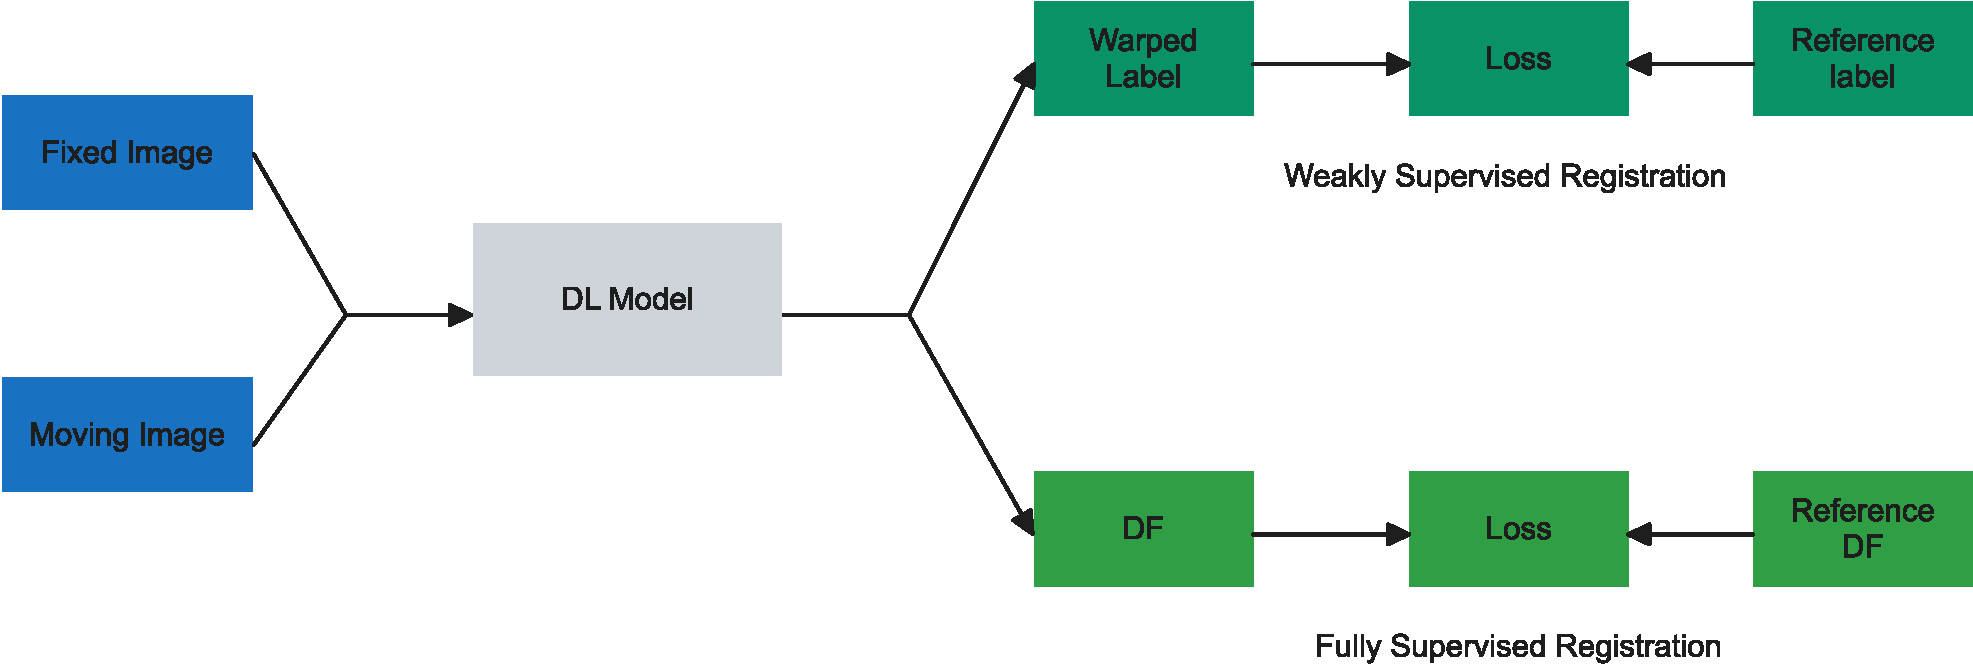
\includegraphics[width=0.9\textwidth]{fig1-Supervised Registration-crop.pdf}
    \caption{有监督配准模型}
    \label{fig:1}
\end{figure}

Miao等人首次采用深度学习算法预测图像的配准变换参数。他们指出现有的配准方法在计算速度和变形范围方面存在局限性,因此他们构建了一个五层的卷积神经网络(CNN)结构,利用CNN回归器直接估计变换参数,从而实现3D CT图像与2D X射线脊柱图像的刚性配准。相较于一些传统的基于强度的配准方法,该方法显著改善了配准效果\cite{miao2016cnn}。在后续研究中\cite{miao2016real},Miao等人提出了一种新的六层CNN网络结构,能够直接基于数字重建射线照片(DRR)和X射线图像来估计变换参数。该方法可以用较少的DRR渲染实现精准的2D/3D配准,且计算效率较高,更适合于实时应用。

Cao等人\cite{cao2018deep}使用了具有3个神经元的基于CNN的模型的输出层,其中每个神经元表示微小斑块中间沿x、y和z轴的运动幅度,能够得到与更传统的方法一样准确的结果。

Yang等人使用基于CNN的U-Net模型学习了具有相同分辨率的大脑MR图像的形变场,并在各种数据集上获得了出色的配准精度\cite{yang2017quicksilver}。

Uzunova等人采用了Flow Net框架\cite{dosovitskiy2015flownet},并使用三种方法生成标准标签数据\cite{uzunova2017training}:仿随机生成、仿射配准生成和统计外观模型(SAM)生成变换。然后,他们利用合成形变场对脑部和心脏的2D MR图像进行了配准。研究表明,在这三种方法中,使用基于SAM生成的标准标签数据进行CNN的学习和训练取得了最优效果。

Fan等人将监督损失与无监督损失相结合,利用双重监督来预测脑部3D MR配准的形变场。他们提出了一个分层双监督的全卷积网络(FCN)\cite{long2015fully}来解决缺少标准标签数据的问题\cite{fan2019birnet},该网络同时使用标准标签数据和图像相似性度量作为两种监督方式。网络的每一层都加入了损失函数,从而使一些层更容易收敛。基于U-net框架\cite{ronneberger2015u},Fan等人引入了间隙填充,提出了名为“BIRNet”的网络架构,该架构使用预测变换与标准标签数据之间的均方误差(MSE)作为损失函数,并结合预先配准的标准标签数据与图像相似性来训练网络。

Cao等人则采用了MR-MR损失和CT-CT损失两种损失进行双重监督配准\cite{cao2018deep},即在同模态内使用图像相似性来进行监督配准。他们在测试阶段直接根据输入的CT和MR图像预测变换场,通过预对齐图像将多模态配准转化为单模态配准,以实现MR-CT配准。此外,他们使用标准标签数据与预测变换扭曲的待配准图像之间的归一化互相关(NCC)作为损失函数。类似地,Liu等人也采用了监督合成变换和无监督图像相似性描述进行训练\cite{liu2019multimodal}。

\subsection{无监督图像配准}

相较于监督学习,基于无监督学习的配准方法就是在训 练学习网络时,只需要提供配准对,不需要标准标签数据(即真实的形变场)。因此,该类方法在训练与测试阶段,均不需要依靠传统的配准方法进行辅助。无监 督配准方法的流程如图\ref{fig:7}。

\begin{figure}[h]
    \centering
    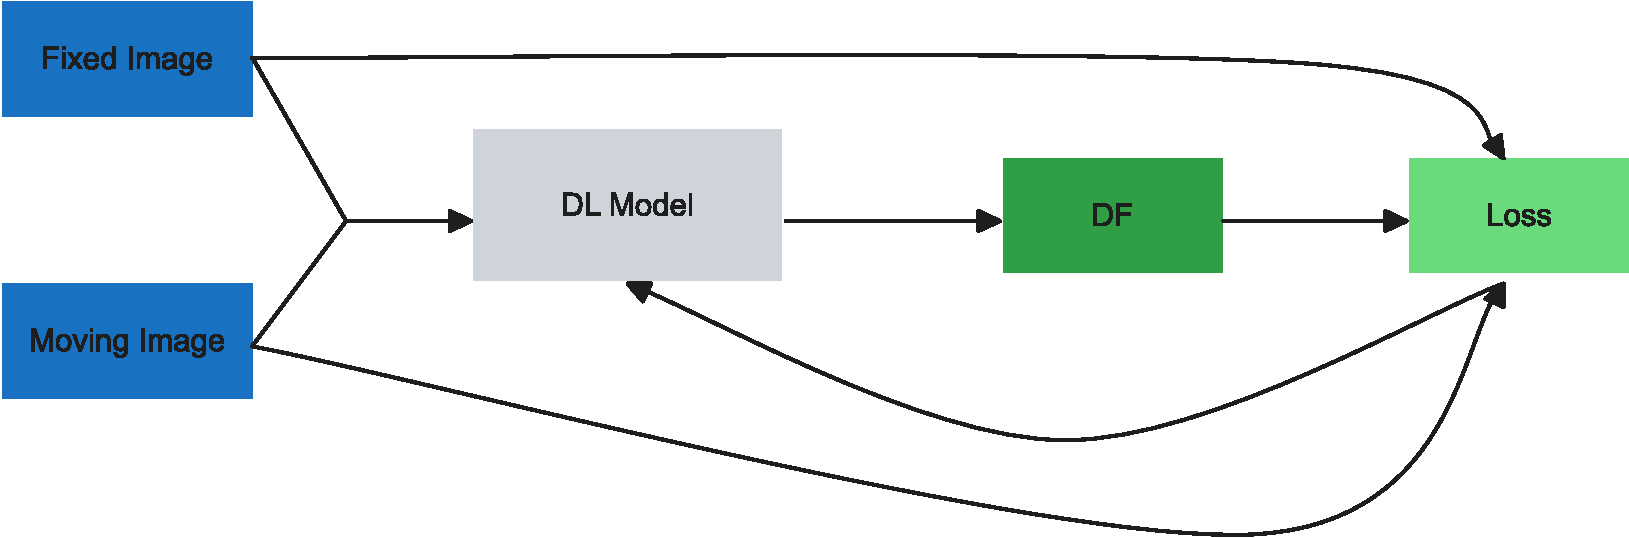
\includegraphics[width=0.9\textwidth]{fig7-unsupervised Registration-crop.pdf}
    \caption{无监督配准模型}
    \label{fig:7}
\end{figure}

de Vos等人提出了一个无监督的图像配准框架DLIR\cite{de2019deep},该框架利用固定图像和移动图像之间的相似性来训练网络,通过优化神经网络间接优化变换参数,预测的变换参数用于构建密集位移矢量场。在另一项研究中,de Vos等人提出了一种深度学习网络“DIRNet”\cite{de2017end},用于可变形图像配准。DIRNet由卷积神经网络回归器、空间变换器和重采样器组成,通过直接优化固定图像和移动图像之间的相似性来学习配准,从而实现心脏MR图像的配准。

Li等人同样利用图像相似性进行配准,通过最大化固定图像和移动图像之间的相似度直接估计图像对之间的空间变换。他们对全卷积网络(FCN)\cite{long2015fully}架构进行了改造,并采用多分辨率策略,以优化和学习在不同分辨率下的空间变化,同时将固定图像与移动图像之间的归一化互相关(NCC)及其他正则项作为损失函数。

相似地,Yoo等人\cite{avants2008symmetric}将卷积自动编码器(CAE)与空间变换网络(STN)\cite{jaderberg2015spatial}相结合,通过计算特征间的相似性,利用CAE以无监督的方式训练网络,实现对神经组织电子显微镜(ssEM)图像的无监督变换估计。

Balakrishnan等人设计了VoxelMorph配准框架\cite{balakrishnan2018unsupervised,balakrishnan2019voxelmorph},该框架由一个配准网络和一个分割网络组成,并在U-Net\cite{ronneberger2015u}的基础上进行了改造。该框架的损失函数结合了图像相似性与分割值的重合度,分割结果在一定程度上提高了配准的准确性。在后续的研究中,Dalca等人利用微分同胚来预测形变场,将均方误差(MSE)作为相似性度量,并与正则项结合构造损失函数,以实现脑部MR图像的无监督配准。

Alexander Bigalke等人提出了一种创新的配准网络RegCST\cite{bigalke2023unsupervised},该方法采用循环自训练策略进行递归训练。这一方法的核心在于其能够通过自我迭代地优化模型,使学习任务特定的特征更加鲁棒,尤其是在处理含噪声数据时。RegCST通过不断地更新和调整特征提取过程,极大地提高了所提取特征的表现力,使得配准结果在各类复杂场景下也能表现出色。此外,该网络在不同的医学成像数据集上进行了验证,展现出了优越的性能和广泛的适用性。

Wang等人提出了一种新颖的无监督配准网络PAN\cite{wang2024pyramid},该网络引入了自注意力机制和金字塔方法,以提高图像配准的效果。具体而言,PAN使用LAT模块,通过多尺度的形变场生成,来精准捕捉不同层次的特征信息。自注意力机制的引入使得模型能够集中关注图像中的关键信息,从而提升整体的配准质量。该网络不仅在保持高效性方面做出了重要贡献,同时也在多项实验中证明了其在各种图像配准任务中的优越性,包括处理高噪声和非刚性变形的数据。

Liu等人则提出了一种全新的无监督医学图像配准互学习范式MutualReg\cite{liu2024mutualreg}。该方法通过引入知识蒸馏机制,将教师网络和学生网络进行循环迭代更新,直到模型收敛为止。以教师网络为指导,学生网络不断吸收和重构知识,从而提高了配准性能。这种互学习的策略在多个医学图像数据集上验证了其有效性,取得了最佳的配准精度,尤其在处理多模态和多样本数据时表现尤为突出。MutualReg不仅优化了模型的学习过程,同时也推动了无监督配准技术的发展,为临床应用提供了更为精确和可靠的工具。


\section{主要研究内容及论文章节安排}

本文一共有七章,其中每章的安排如下:

第一章:绪论。首先介绍了基于金字塔结构与迭代优化的脑部医学图像配准的研究背景及意义;其次,介绍了医学图像配准的国内外研究现状;最后,介绍了本文的主要研究内容和章节安排。

第二章:训练与验证数据集介绍与选用。首先,介绍了用于脑部配准的MRI数据集及各自特点;其次,介绍了用于神经网络训练过程的数据集选用及预处理过程;再次,介绍了用于验证神经网络性能的数据集选用与预处理过程;最后,介绍了医学图像配准常用的评估,如定性评估和定量评估。

第三章:基于MutualReg互学习配准框架设计。首先,介绍了基于互学习的MutualReg框架及其训练流程;其次,介绍了本文对于MutualReg框架教师网络及学生网络的选用与介绍。

第四章:基于PAN网络的改进与预训练。首先,介绍了基于金字塔结构与自注意力机制的PAN网络的总体框架;然后,介绍了将PAN网络与训练数据集相适配的逻辑及实现;再次,介绍了对于PAN网络训练过程中损失函数的设计与改进;最后,通过与原始网络在验证数据集上的配准对比实验验证了PAN网络预训练阶段的性能与改进方法的有效性。

第五章:基于RegCST网络的改进与预训练。首先,介绍了基于CNN和迭代优化的RegCST网络的总体框架;然后,介绍了将RegCST网络与训练数据集适配的逻辑及实现;其次,介绍了RegCST网络在训练过程中的损失函数设计及改进方法;最后,通过在验证数据集上与原始网络的配准对比实验验证了改进方法的有效性与预训练阶段RegCST网络的性能。

第六章:VRC模块消融分析。首先,介绍了对于VRC模块消融实验的目的;然后,介绍了VRC模块消融实验的设计;最后,通过在验证数据集上的配准对比实验验证VRC模块对于提升互学习配准性能的有效性。

第七章:互学习优化。首先,介绍了基于MutualReg的互学习优化实验设计;然后,通过不同互学习阶段网络在验证数据集上的配准对比实验验证了互学习对于提升配准性能的有效性。

\chapter{训练与验证数据集介绍与选用}

\section{训练数据集选用}

在预训练和递归互学习阶段,采用Learn2Reg(L2R)挑战赛的大规模无监督脑部MRI图像配准(LUMIR)数据集进行训练。该数据集包括专注于无监督图像配准的OpenBHB\cite{dufumier2022openbhb}数据集,包含来自10个不同公共数据集的T1加权脑MRI扫描;以及部分源自AFIDs项目的OASIS\cite{marcus2007open}数据集。训练数据集中包含3384张图像。其核心特点是仅提供大量的无标注原始图像,不限制具体的图像配对方式,由参与者自由创建图像对,为深入的无监督学习提供了高度的灵活性。因此,在使用LUMIR数据集进行训练之前需要根据其图像数据创建训练图像对。

为了充分利用大规模数据集的数据量优势,并且防止过多质量较差数据对于模型性能以及训练过程中收敛困难的问题,在预训练阶段,采用基于均方误差的相似性指标建立训练图像对。具体而言,图像对建立过程如下:

\begin{enumerate}
    \item 对于每两对图像,计算其MSE指标作为这两张图像的相似度指标
    \item 依次选择相似度最高的两张图像进行配对
    \item 直到每张图像都有与之配对的图像
    \item 对每对图像进行快速仿射对齐
\end{enumerate}

同时,为了避免过多低质量或无意义的图像对参与训练,并且提高配对数据的整体质量,每张图像被限制最多与2张图像进行配对。经过筛选后,总共得到了1835对训练图像。这一策略通过优先选择解剖结构对齐程度较高的图像对,降低了初始训练的优化复杂度,同时通过配对数量限制避免模型过度依赖局部相似模式,为后续无监督学习提供了稳定且多样化的数据基础。

这样做有以下的优势

\begin{itemize}
    \item \textbf{减低训练初期的优化难度}:高相似度图像对之间的形变场相对于低相似度图像对之间的形变场通常复杂度较小,可为模型提供更为平滑的优化目标,避免梯度方向剧烈波动导致初期训练难度增加导致模型收敛困难。
    \item \textbf{隐式数据增强}:严格限制图像之间的一一配对可能限制训练样本的多样性,为此将每张图像的配对数量放宽至2,增加训练数据的多样性;并且也能够控制训练图像对数,防止训练时间过长。
    \item \textbf{降低模型收敛困难的风险}:通过相似性筛选,能够保证训练样本的相似度,防止随机配对导致部分相似度低的图像参与训练影响模型性能以及出现收敛困难的风险。
\end{itemize}

\section{验证数据集选用}

LUMIR测试集包含590张脑部MRI图像,但缺乏分割标签与解剖标记点信息,可以用来测试最终模型产生位移场的平滑度指标,但是无法用于评价配准精度的Dice指标的测试。为此,选用同样为脑部MRI配准任务的LPBA40数据集作为课题的验证数据集。LPBA40数据集包含40例健康受试者的3D脑MRI扫描数据,每例数据均附带56个脑区的手动精细标注,涵盖海马体、丘脑等关键解剖结构,能够用于Dice指标的测试。

为了保证评价的严谨性,在LPBA40数据集测预处理过程中,对其中的图像进行N4偏置场校正与Z-Score强度归一化。同时对训练数据也做同样的处理,避免因为两个数据集强度分布不一致对最终评价结果产生影响。

此外,测试阶段采用双重验证机制:首先通过可视化叠加展示配准前后的解剖结构对齐效果,定性评估形变场的合理性;随后基于Dice系数和平滑性指标定量分析模型性能。该预处理框架通过数据标准化与空间对齐,在兼顾数据质量与多样性的同时,充分利用了大规模无监督数据的潜力。LUMIR数据集在预训练阶段提供了稳定且丰富的形变模式,LPBA40数据集则为精确的配准精度评估提供了坚实基础。双重验证机制既能定性展示模型在解剖结构对齐上的效果,又可通过多指标(Dice、平滑度)定量分析模型的优缺点,从而为后续的模型迭代与改进提供全面、可靠的依据。

\section{医学图像配准的评估}

医学图像配准的评估分为两种:定性评估和定量评估。其中定性评估容易受主观影响,因此在评判中一般以定量评估为主,定性评估作为辅助。

\subsection{定性评估}

定性评估主要分为两种:可视化评估和差分图像评估。

\paragraph{可视化评估}

可视化评估主要依靠肉眼观察对配准后图像与固定图像的相似性进行评估。如图\ref{fig:c2-1}、\ref{fig:c2-2}、\ref{fig:c2-3},可以看出,经过配准过后得到的配准图像与固定图像更为相似,因此认为该配准效果较好。

\begin{figure}[h]
    \centering
    \begin{minipage}{0.3\textwidth}
        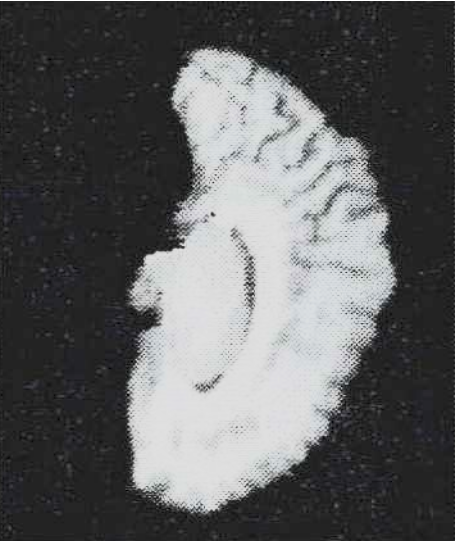
\includegraphics[width=\textwidth]{c2-fiximg.png}
        \caption{固定图像}
        \label{fig:c2-1}
    \end{minipage}
    \begin{minipage}{0.3\textwidth}
        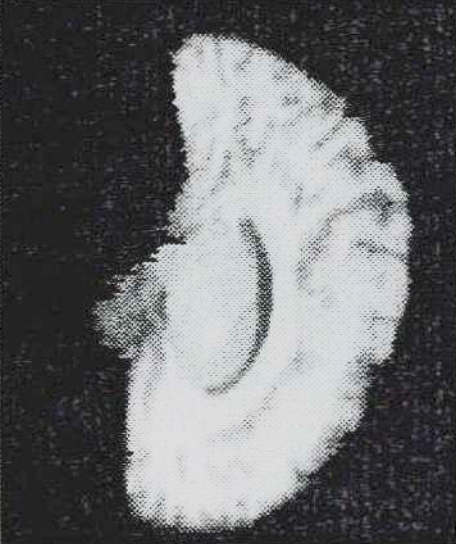
\includegraphics[width=\textwidth]{c2-moveimg.png}
        \caption{浮动图像}
        \label{fig:c2-2}
    \end{minipage}
    \begin{minipage}{0.3\textwidth}
        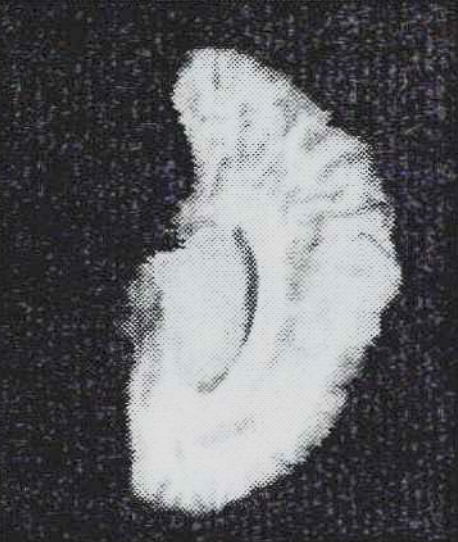
\includegraphics[width=\textwidth]{c2-regimg.png}
        \caption{配准图像}
        \label{fig:c2-3}
    \end{minipage}
\end{figure}

在有分割标签时,可将配准后的标签叠加在固定图像上以便于更好的观察两幅图像特定解剖结构的相似性,如图\ref{fig:c2-4}。

\begin{figure}[h]
    \centering
    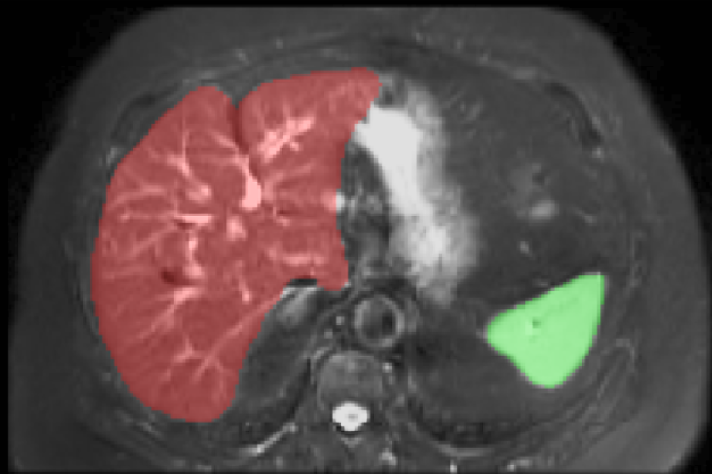
\includegraphics[width=0.9\textwidth]{c2-markedimg.png}
    \caption{带分割标签的可视化图像}
    \label{fig:c2-4}
\end{figure}

\paragraph{差分图像评估}

相较于肉眼观察,差分图的方式更为直观。将配准图像与固定图像做差分即可得到差分图,差分图越接近黑色,表示配准效果越好,反之效果越差。

\begin{figure}[h]
    \centering
    \begin{minipage}{0.4\textwidth}
        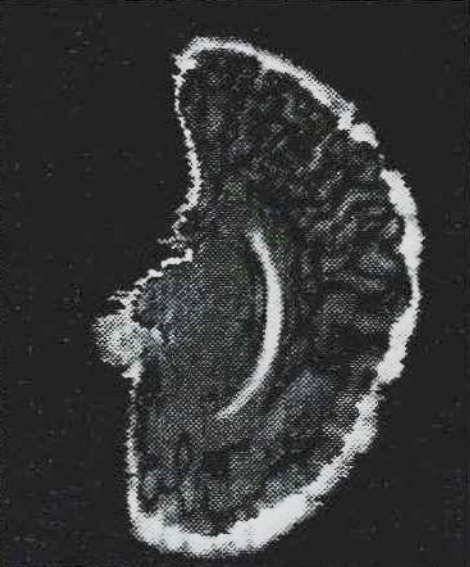
\includegraphics[width=\textwidth]{c2-imgdiff1.png}
        \caption{浮动图像差分图}
        \label{fig:c2-5}
    \end{minipage}
    \begin{minipage}{0.4\textwidth}
        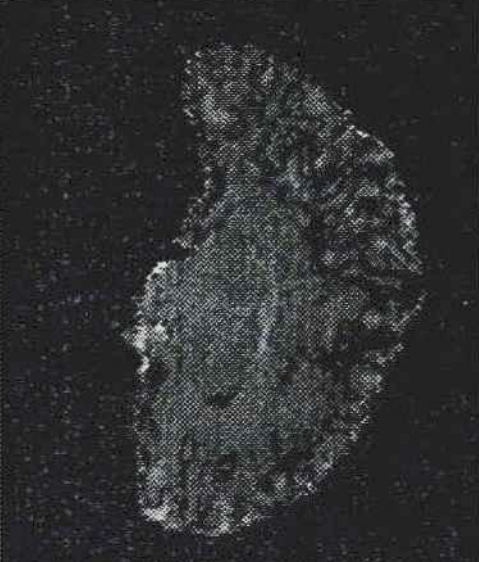
\includegraphics[width=\textwidth]{c2-imgdiff2.png}
        \caption{配准后图像差分图}
        \label{fig:c2-6}
    \end{minipage}
\end{figure}

图\ref{fig:c2-5}是浮动图像与固定图像的差分图,可以看出在大脑边缘两张图像并不对齐,有较多的白色区域,表明固定图像与浮动图像在该区域相似性不佳。图\ref{fig:c2-6}是经过配准后的配准图像与固定图像的差分图,图像基本呈现黑色,尤其在边缘部分,表明配准后图像已经基本对齐。

\subsection{定量评估}

定量评估主要分为两类:评价配准精度的指标如Dice系数;评价形变场平滑度的指标如雅可比行列式、SDlogJ。

\paragraph{Dice系数}

Dice系数主要用于评估固定图像与配准后图像在对应解剖区域的重叠程度,Dice系数的计算如公式\ref{eq:c2-1}。

\begin{equation}
    \mathrm{Dice}(A,B)=2\times\frac{\left|A\cap B\right|}{\left|A\right|+\left|B\right|}
    \label{eq:c2-1}
\end{equation}

其中$A$和$B$分别表示固定图像与配准后图像相对应的解剖区域,Dice系数越接近1,代表配准后在对应解剖区域的相似性越高,配准精度越高,反之配准精度越低。

\paragraph{雅可比行列式}

雅可比行列式常用于评价形变场的平滑性。以三维数据为例,在形变场上的每个点的雅可比行列式计算如公式\ref{eq:c2-2}:

\begin{equation}
    \centering
    \det(J(i,j,k))=\begin{vmatrix}\frac{\partial i}{\partial x} & \frac{\partial j}{\partial x} & \frac{\partial k}{\partial x} \\\frac{\partial i}{\partial y} & \frac{\partial j}{\partial y} & \frac{\partial k}{\partial y} \\\frac{\partial i}{\partial z} & \frac{\partial j}{\partial z} & \frac{\partial k}{\partial z}\end{vmatrix}
    \label{eq:c2-2}
\end{equation}

\paragraph{SDlogJ}
SDlogJ(Standard Deviation of Logarithmic Jacobian determinant)用于量化形变场局部体积变化的离散程度。其计算基于雅可比行列式,具体过程如公式\ref{eq:sdlogj}所示:

\begin{equation}
    \centering
    \text{SDlogJ} = \sqrt{ \frac{1}{N} \sum_{(x,y,z) \in \Omega} \left( \log \det(J(x,y,z)) - \mu_{\log J} \right)^2 }
    \label{eq:sdlogj}
\end{equation}

其中:
\begin{itemize}
    \item $\det(J(x,y,z))$为点$(x,y,z)$的雅可比行列式,计算方法如公式\ref{eq:c2-2}所示
    \item $\mu_{\log J} = \frac{1}{N} \sum_{(x,y,z) \in \Omega} \log \det(J(x,y,z))$为有效区域内对数雅可比行列式的均值
    \item $N$为满足$\det(J) > 0$的体素总数,排除$\det(J) \leq 0$的折叠区域
\end{itemize}

该指标通过标准差度量$\log \det(J)$的离散度,对异常体积变化具有更高敏感性。SDlogJ趋近于零时表明形变场具有均匀的体积变化特性,较大值则提示局部存在剧烈膨胀或收缩。

\section{本章小结}

本章阐述了医学图像配准研究中训练与验证数据集的构建策略及评估方法体系。针对无监督学习框架对大规模数据的需求,选用LUMIR挑战赛的3384张脑部MRI图像作为训练数据源,通过基于均方误差的相似性筛选机制构建1835对高质量训练样本。为克服LUMIR测试集缺乏标注的局限性,引入LPBA40数据集作为验证基准,其40例含56个脑区精细标注的MRI数据,为定量评估提供了可靠的解剖对齐参照。

在数据预处理环节,采用N4偏置场校正与Z-Score强度归一化的标准化流程,确保训练与验证数据的强度分布一致性,消除跨数据集偏差对评估结果的干扰。

在评估方法层面,介绍了定性分析与定量指标的多维度评价体系。定性评估通过配准图像与固定图像的叠加可视化、解剖标记融合显示以及差分图分析,直观呈现形变场的空间合理性;定量评估则基于Dice系数衡量关键解剖结构的重叠精度,结合雅可比行列式及其对数标准差(SDlogJ)量化形变场的拓扑保持能力与局部平滑特性。


\chapter{基于 MutualReg 互学习配准框架设计}

\section{MutualReg互学习配准框架介绍}

\section{MutualReg互学习配准框架介绍}

MutualReg\cite{liu2024mutualreg}提出了一种基于互学习(Mutual Learning, ML)的无监督医学图像配准范式。其核心理念是,任何网络都可以通过互学习(ML)从自身的无监督损失和另一个网络的有监督损失中进行递归学习。其有监督损失是通过知识蒸馏(KD)机制实现的。MutualReg的目标是通过互学习整合多种损失信息,如图\ref{fig:2}所示。具体而言,MutualReg的训练过程为:

\begin{enumerate}
    \item 在第一阶段,使用常见的无监督学习方法对教师和学生网络进行预训练
    \item 学生和教师网络分别在第二和第三阶段通过相互学习进行微调
    \item 递归训练学生和教师网络,直到收敛
\end{enumerate}

在架构设计上,教师网络与学生网络可采用异构结构以增强伪位移场的多样性与准确性。训练过程中,网络通过两种损失函数协同优化:其一为基于图像相似性与位移场平滑性正则化的无监督损失;其二为教师网络生成的位移场对学生网络的知识蒸馏监督损失。为避免低质量伪标签干扰,VRC模块通过比较$T$与$S$生成的变形场对固定图像的匹配精度,生成掩码,仅保留教师网络中更可靠的体素位置用于监督学习。

\begin{figure}[h]
    \centering
    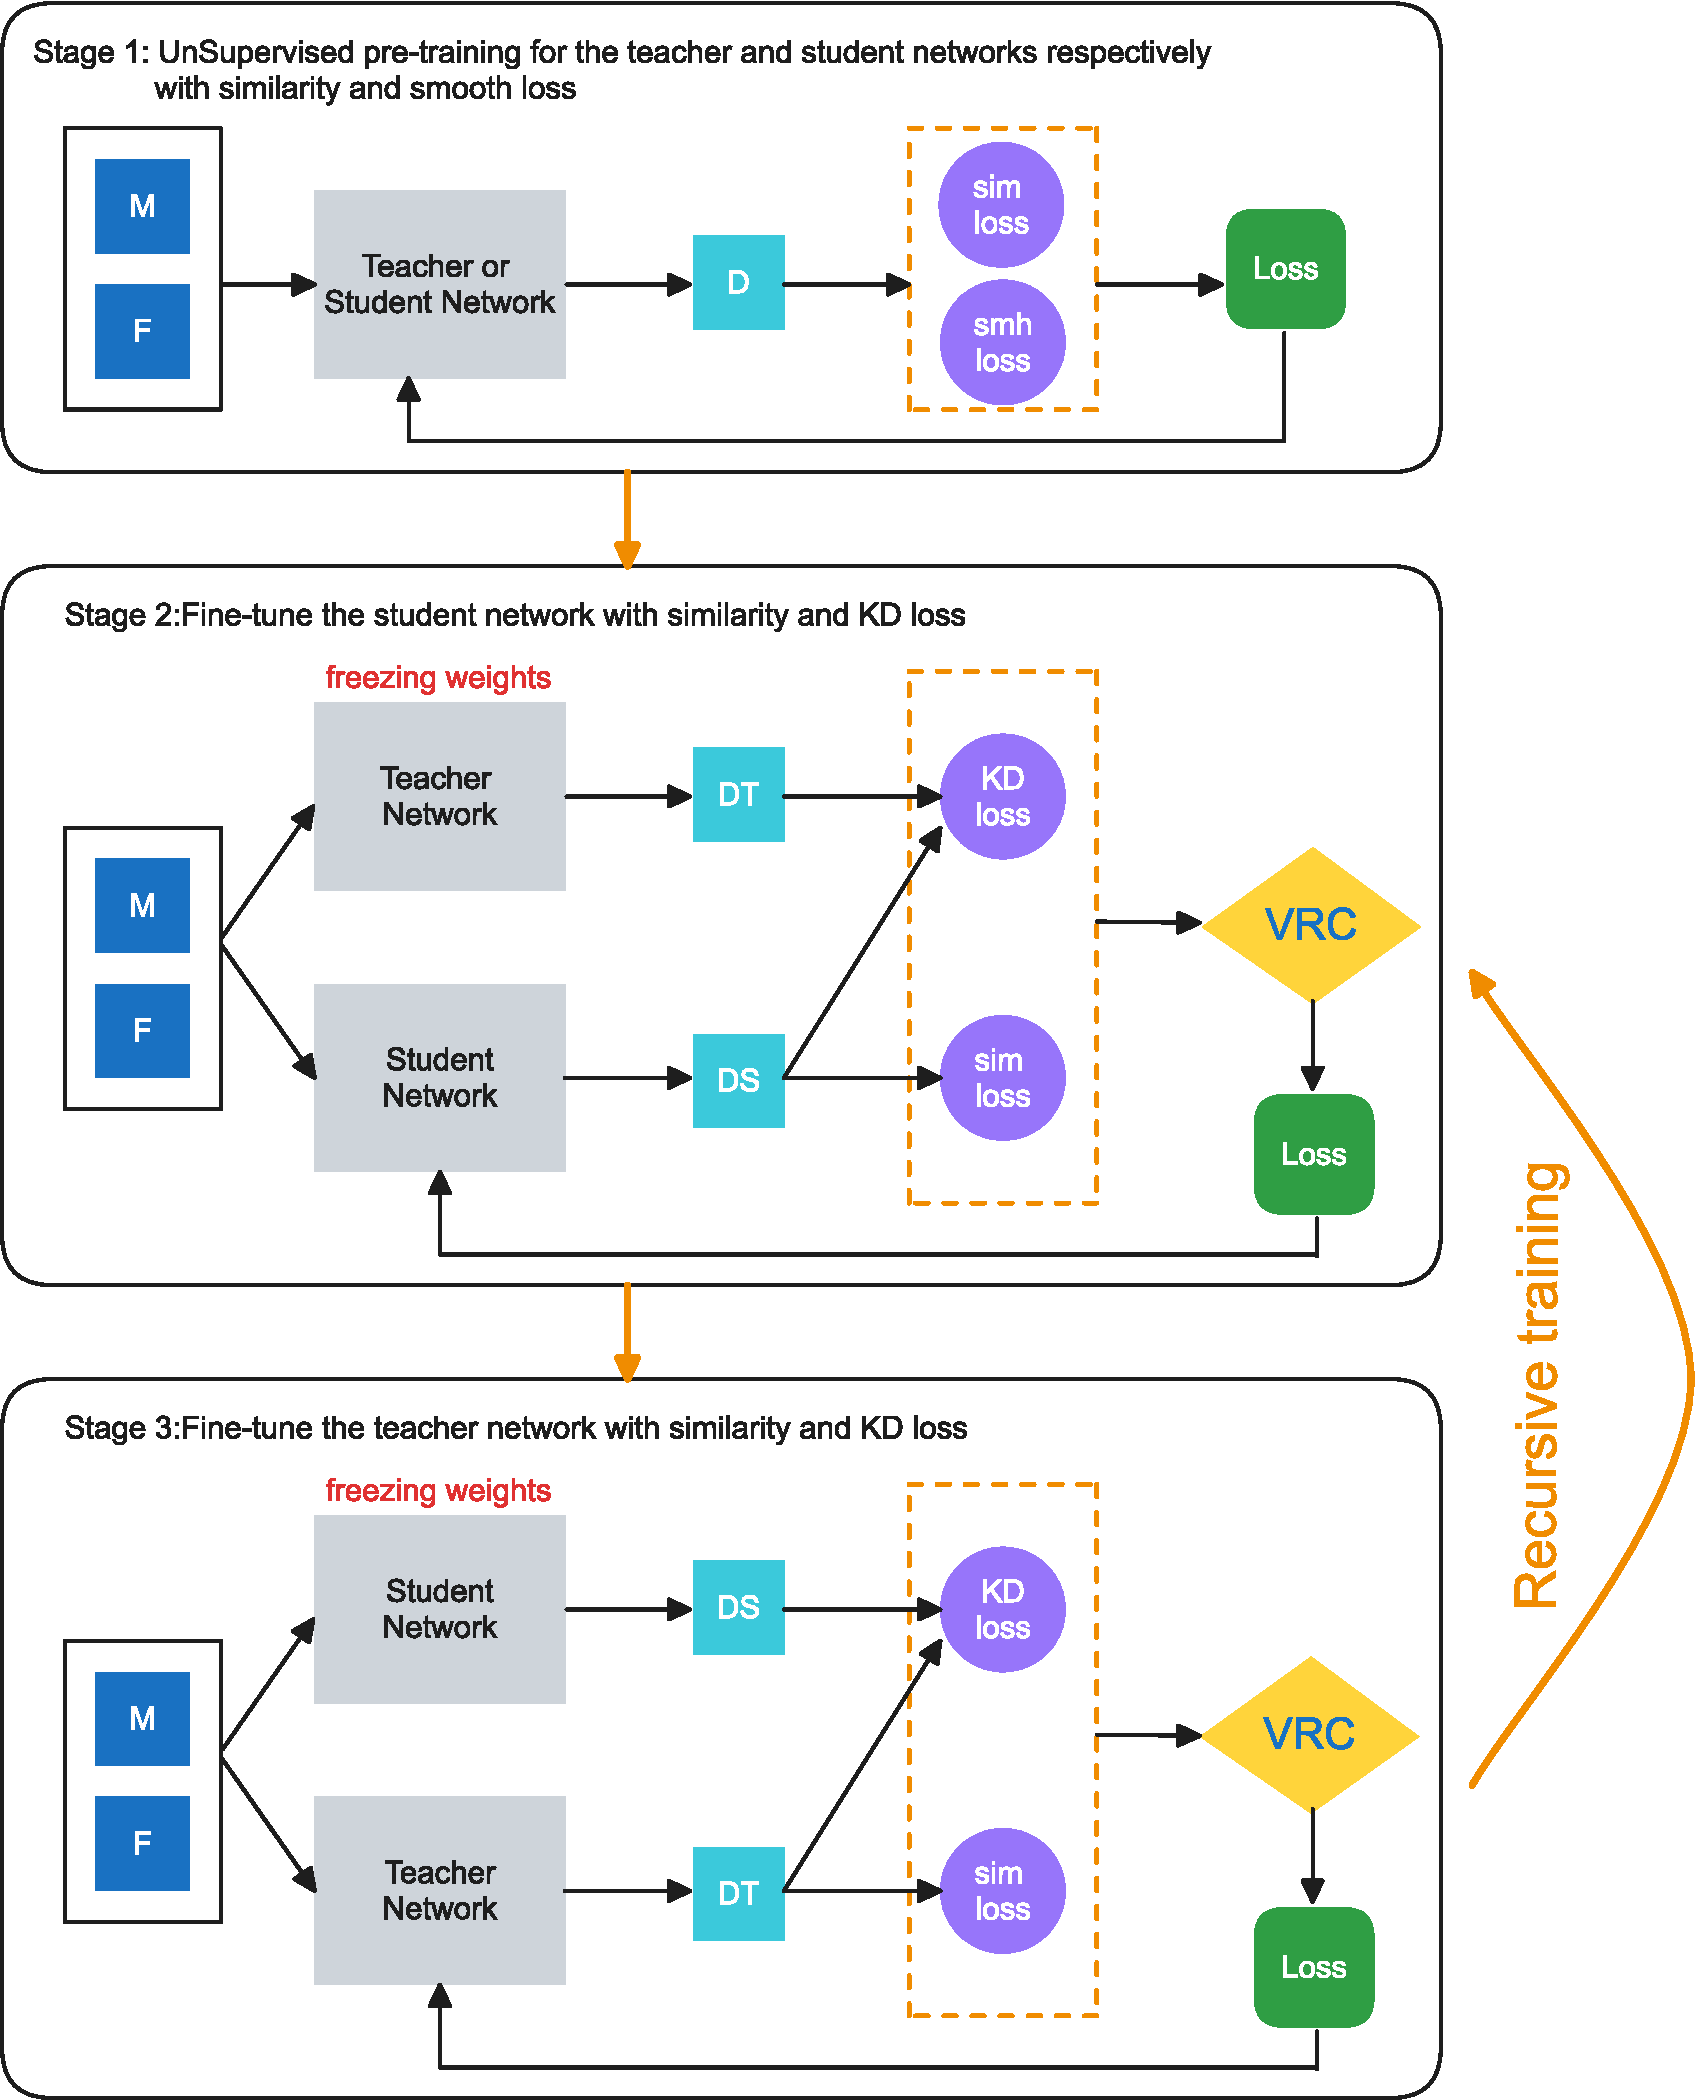
\includegraphics[width=0.9\textwidth]{fig2-mutualreg-crop.pdf}
    \caption{MutualReg的详细框架}
    \label{fig:2}
\end{figure}



本文基于Liu等人所提出的互学习配准范式\cite{liu2024mutualreg},旨在通过递归训练融合基于金字塔和自注意力机制的PAN网络\cite{wang2024pyramid}与基于CNN架构的RegCST网络\cite{bigalke2023unsupervised}。将基于金字塔和自注意力机制的PAN网络选为教师网络,配合基于CNN架构的RegCST网络\cite{bigalke2023unsupervised}作为学生网络。这一选择旨在充分挖掘两种网络的各自优势,以实现更加高效的医学图像配准。

\section{教师网络介绍}

PAN网络\cite{wang2024pyramid}是一种用于医学图像配准的无监督深度学习方法,通过结合双流金字塔编码器和多头局部注意力Transformer解码器,有效解决了传统卷积神经网络特征增强不足及Transformer信息冗余的问题。编码器采用通道注意力机制增强多层次特征表示,解码器通过局部注意力Transformer分析运动模式并生成平滑变形场,同时引入正交正则化减少特征冗余以提升运动模式建模能力。其网络架构如图\ref{fig:4}。

\begin{figure}[h]
    \centering
    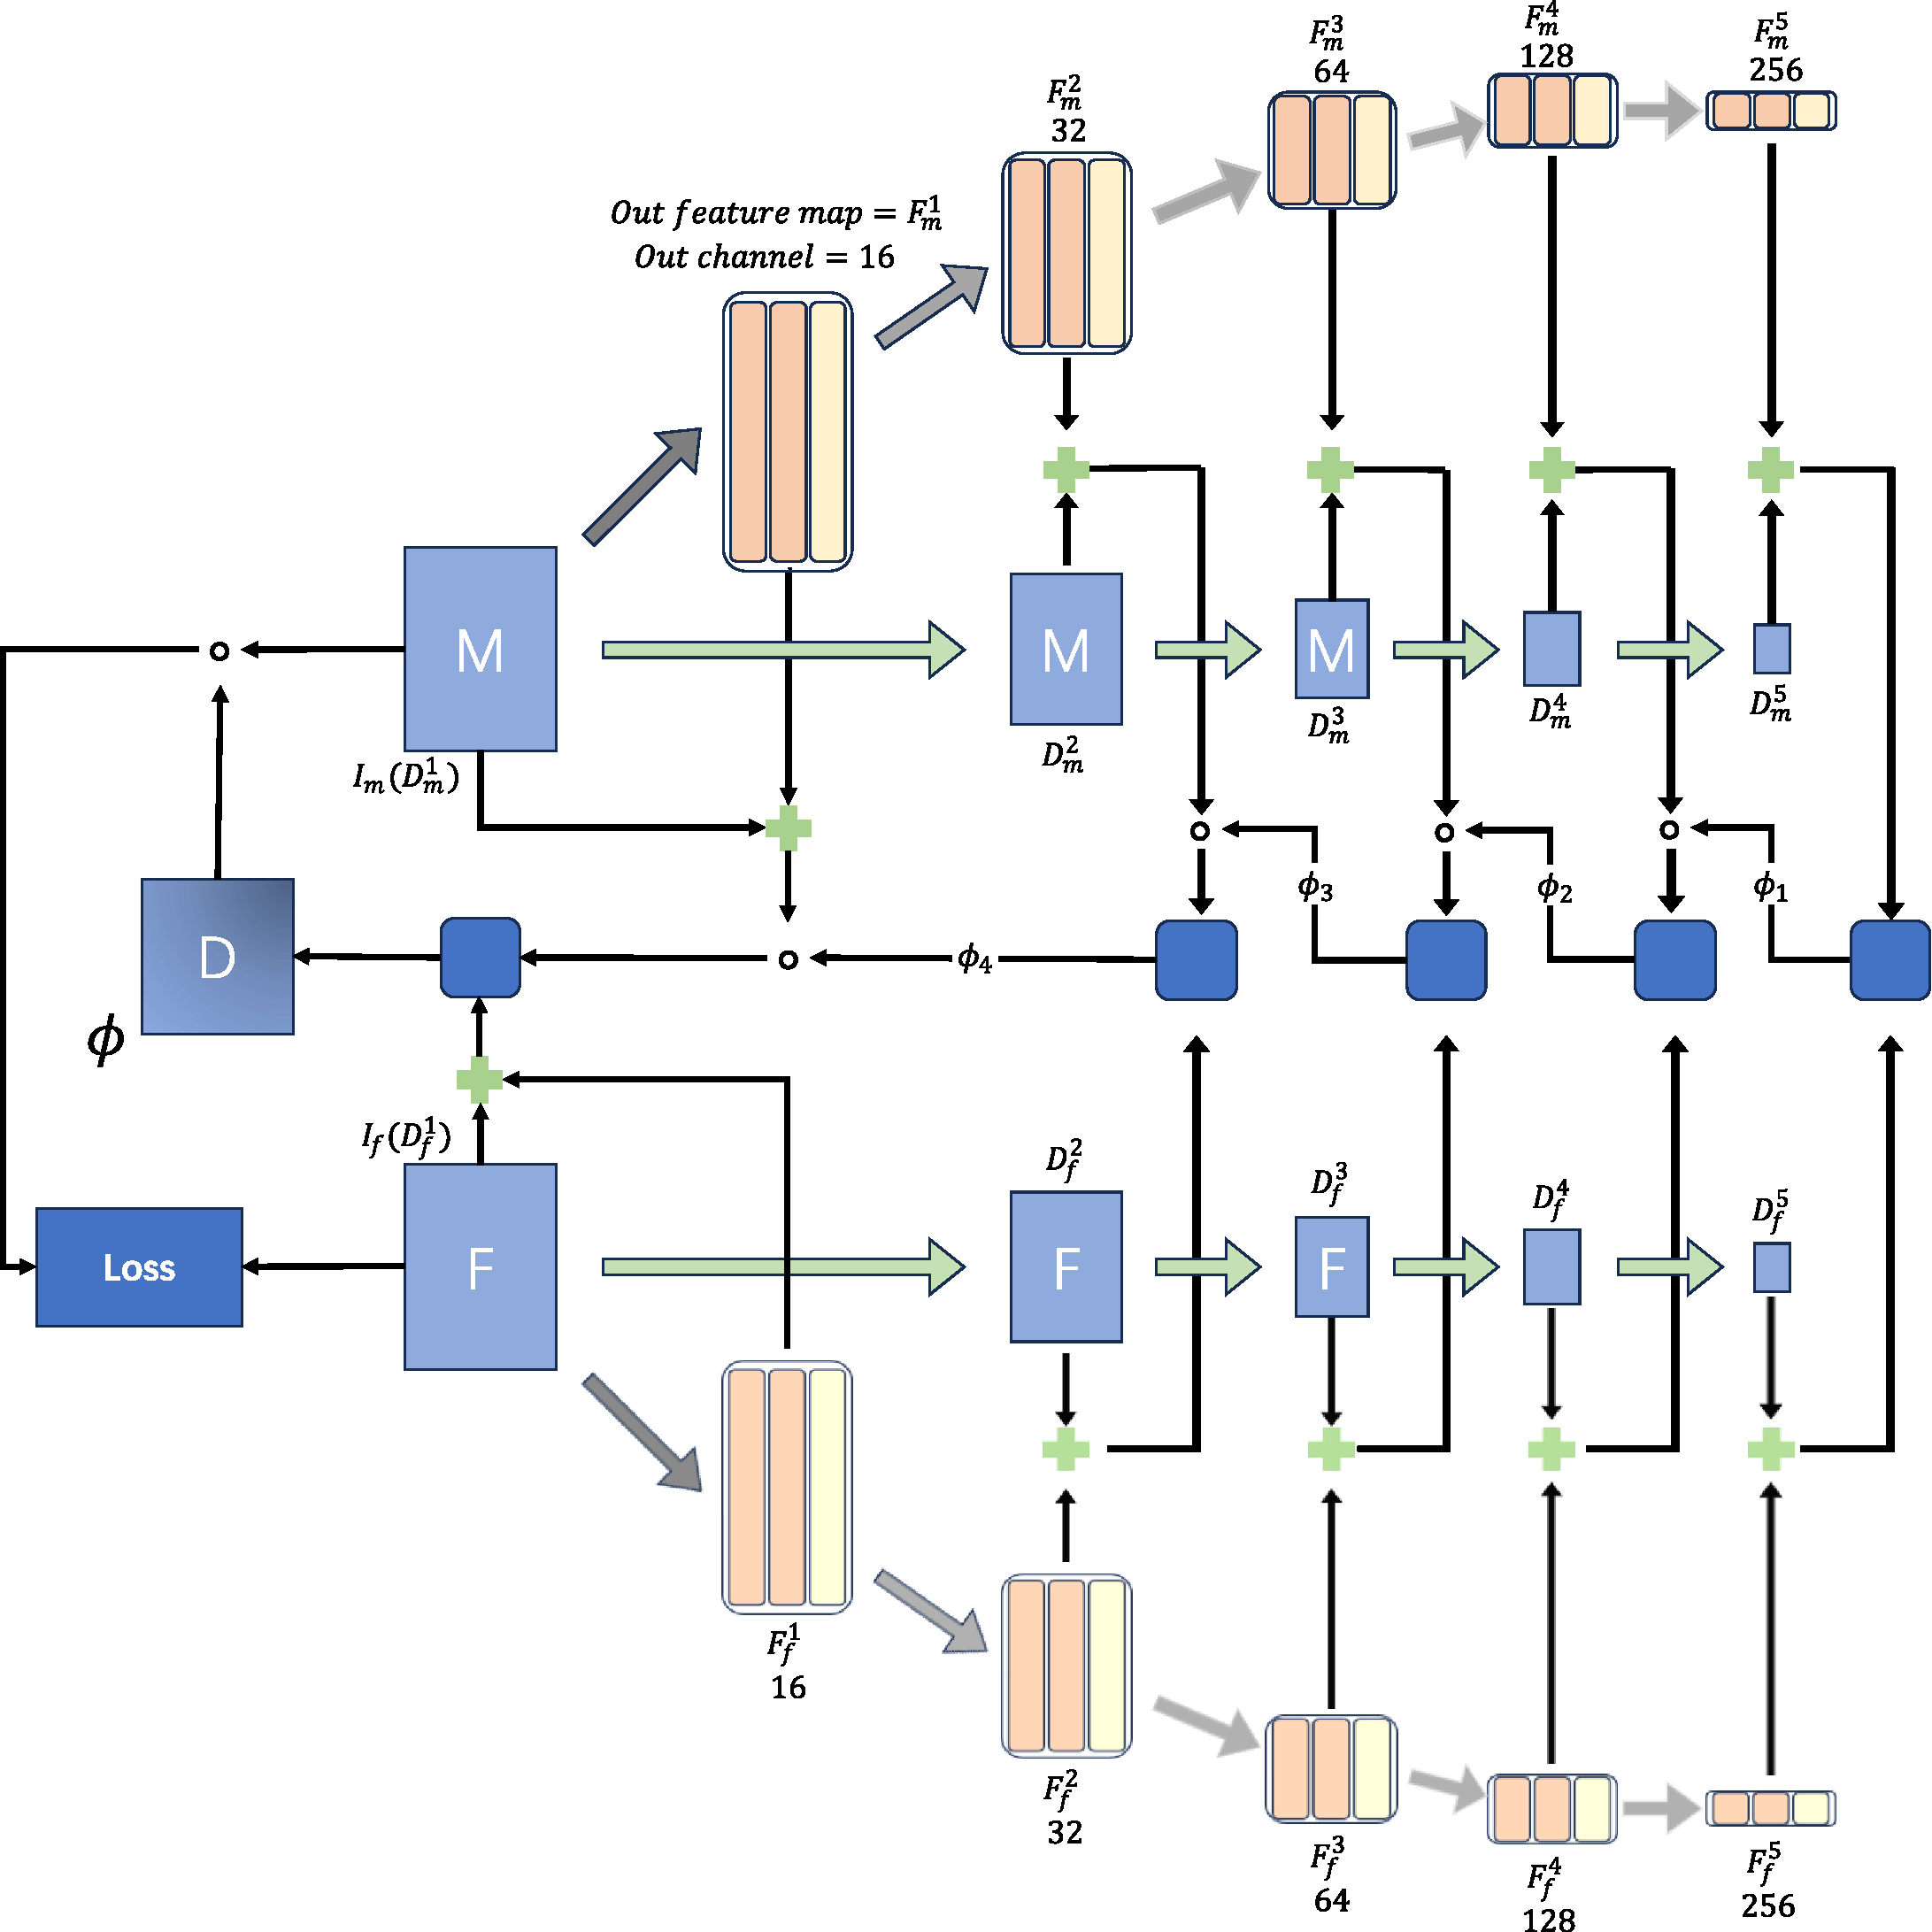
\includegraphics[width=0.9\textwidth]{fig4-PAN-crop.pdf}
    \caption{PAN网络架构}
    \label{fig:4}
\end{figure}

其网络主要由双流金字塔编码器和局部注意力Transformer解码器组成。

双流权重共享的金字塔编码器使用运动图像$I_m$和固定图像$I_f$作为输入,并通过一系列通道注意力块生成两组分组特征:$\{F_m^1,F_m^2,F_m^3,F_m^4,F_m^5\}$和$\{F_f^1,F_f^2,F_f^3,F_f^4,F_f^5\}$。同时,$I_m$和$I_f$经过下采样生成图像集$\{D_m^1,D_m^2,D_m^3,D_m^4,D_m^5\}$和$\{D_f^1,D_f^2,D_f^3,D_f^4,D_f^5\}$,并于相对对应的特征图进行对齐。

对于每个通道注意力块,使用两个卷积块(每个块都有一个$3\times3\times 3$的卷积层、一个实例归一化层\cite{ulyanov2016instance}和一个LeakyReLU激活层)和一个压缩和激励(SE)块\cite{hu2018squeeze}。SE块通过结合全局信息动态优化特征图,促进编码器生成更具代表性的特征。

在解码器部分,利用局部注意力Transformer(LAT),来解析特征图并推导出形变场。首先将$(F_m^5,D_m^5)$和$(F_f^5,D_f^5)$输入LAT模块,以分析形变并生成初始形变场$\phi_1$。之后利用$\phi_1$对$(F_m^4,D_m^4)$进行形变,并将$(F_m^4\circ \phi_1,D_m^4\circ\phi_1 )$和$(F_f^4,D_f^4)$做为后续LAT的输入,生成$\phi_2$。类似的,生成$\phi_3,\phi_4$和最终的形变场$\phi$。

作为教师网络,PAN网络不仅能引导学生网络识别和关注关键区域,还能通过其强大的特征选择能力,促进学生网络的学习。

\subsection{局部注意力Transformer模块}

局部注意力Transformer模块用于生成每个下采样层的形变场。具体而言将编码器特定层的运动图像特征图、固定图像特征图及其相应的降采样图像分别表示为 \( F_m \)、\( F_f \)、\( D_m \) 和 \( D_f \)。之后,将 \( (F_f, D_f) \) 和 \( (F_m, D_m) \) 在通道维度上进行连接。然后,连接后的特征通过线性投影(LP)和层归一化(LayerNorm,LN)计算查询(Q)和键(K),具体表达如下:

\begin{equation}
    Q = LN(LP(\text{concat}(F_f, D_f)))
\end{equation}

\begin{equation}
    K = LN(LP(\text{concat}(F_m, D_m)))
\end{equation}

对于多头注意力机制,\( Q \in \mathbb{R}^{S \times h \times w \times l \times \frac{c}{S}} \) 和 \( K \in \mathbb{R}^{S \times h \times w \times l \times \frac{c}{S}} \) 可以按注意力头的数量 \( S \) 划分为 \( \{ Q_1, Q_2, \ldots, Q_S \} \) 和 \( \{ K_1, K_2, \ldots, K_S \} \),其中 \( c \) 是通道数。那么,第 \( s \) 个注意头的局部注意力图 \( LA \) 可以通过以下公式计算:

\begin{equation}
    LA_s = \text{softmax}\left(Q_s \cdot K_s^T + P_s\right)
\end{equation}

其中 \( N(x) \) 表示体素 \( x \) 的 \( N \times N \times N \) 邻域,\( P \in \mathbb{R}^{S \times N \times N} \) 是可学习的相对位置偏差。

局部注意力图 \( LA \) 蕴含了不同运动模式的信息。因此,可以利用局部注意力图对规则形变场进行加权,以生成一系列可能的形变子场:

\begin{equation}
    \phi_s = LA_s \cdot V
\end{equation}

其中 \( V \in \mathbb{R}^{n \times n \times n} \) 表示邻域质心的相对位置坐标。

最后,通过卷积层合并来自每个注意头的形变子场 \( \{ \phi_1, \phi_2, \ldots, \phi_S \} \),以在第 \( t \) 个解码层生成最终的形变场 \( \phi_t \in \mathbb{R}^{h \times w \times l \times 3} \)。

在多头学习中会出现潜在同质性问题。潜在同质性可能导致信息冗余,使得多个头部学习到相似的特征,从而降低模型的区分能力和整体性能。这种同质化会导致特征表达不足,影响模型在多类别任务中的判别性,同时也使训练效率降低,浪费计算资源。

因此,为了解决多头LAT学习内容的潜在同质性,PAN网络在LAT模块中使用正交损失$L_{orth}$对特征学习进行正则化\cite{brock2016neural}。

首先将查询(Q)和键(K)根据注意力头的维度转换为平面向量,形成一个矩阵 \( W \in \mathbb{R}^{S \times u} \)(其中 \( u = h \cdot w \cdot l \cdot c_s \))。在获得矩阵 \( W \) 之后,对每个头部所表示的向量进行归一化处理,并与其转置相乘。最终,正交性损失 \( L_{\text{orth}} \) 可以通过以下公式计算:
\begin{equation}
    L_{\text{orth}} = L_{\text{MSE}}\left(\text{Norm}(W) \cdot \text{Norm}(W)^T, I\right)
\end{equation}

其中,\( I \) 是单位矩阵,\( L_{\text{MSE}} \) 是均方误差(即 \( l_2 \) 范数)的计算。

\section{学生网络介绍}

RegCST\cite{bigalke2023unsupervised}是一种基于循环自训练策略的无监督3D医学图像配准框架,其核心架构通过深度融合深度特征提取网络与可微分优化算法,实现了从伪标签生成到网络参数更新的闭环优化。如图\ref{fig:regcst}所示,该网络主要由特征提取模块、优化器模块及自训练机制三部分构成。特征提取模块采用标准3D卷积神经网络,包含6层卷积操作,每层卷积核尺寸为$3 \times 3 \times 3$,通道数逐层递增(32、64、128),并通过步长为2的下采样将输入图像分辨率缩减至原始尺寸的1/8。网络末端通过$1 \times 1 \times 1$卷积将固定图像与移动图像的特征映射至16维空间,并输入相关性层计算多尺度位移匹配响应,为后续优化提供高判别性特征表示。

\begin{figure}[h]
    \centering
    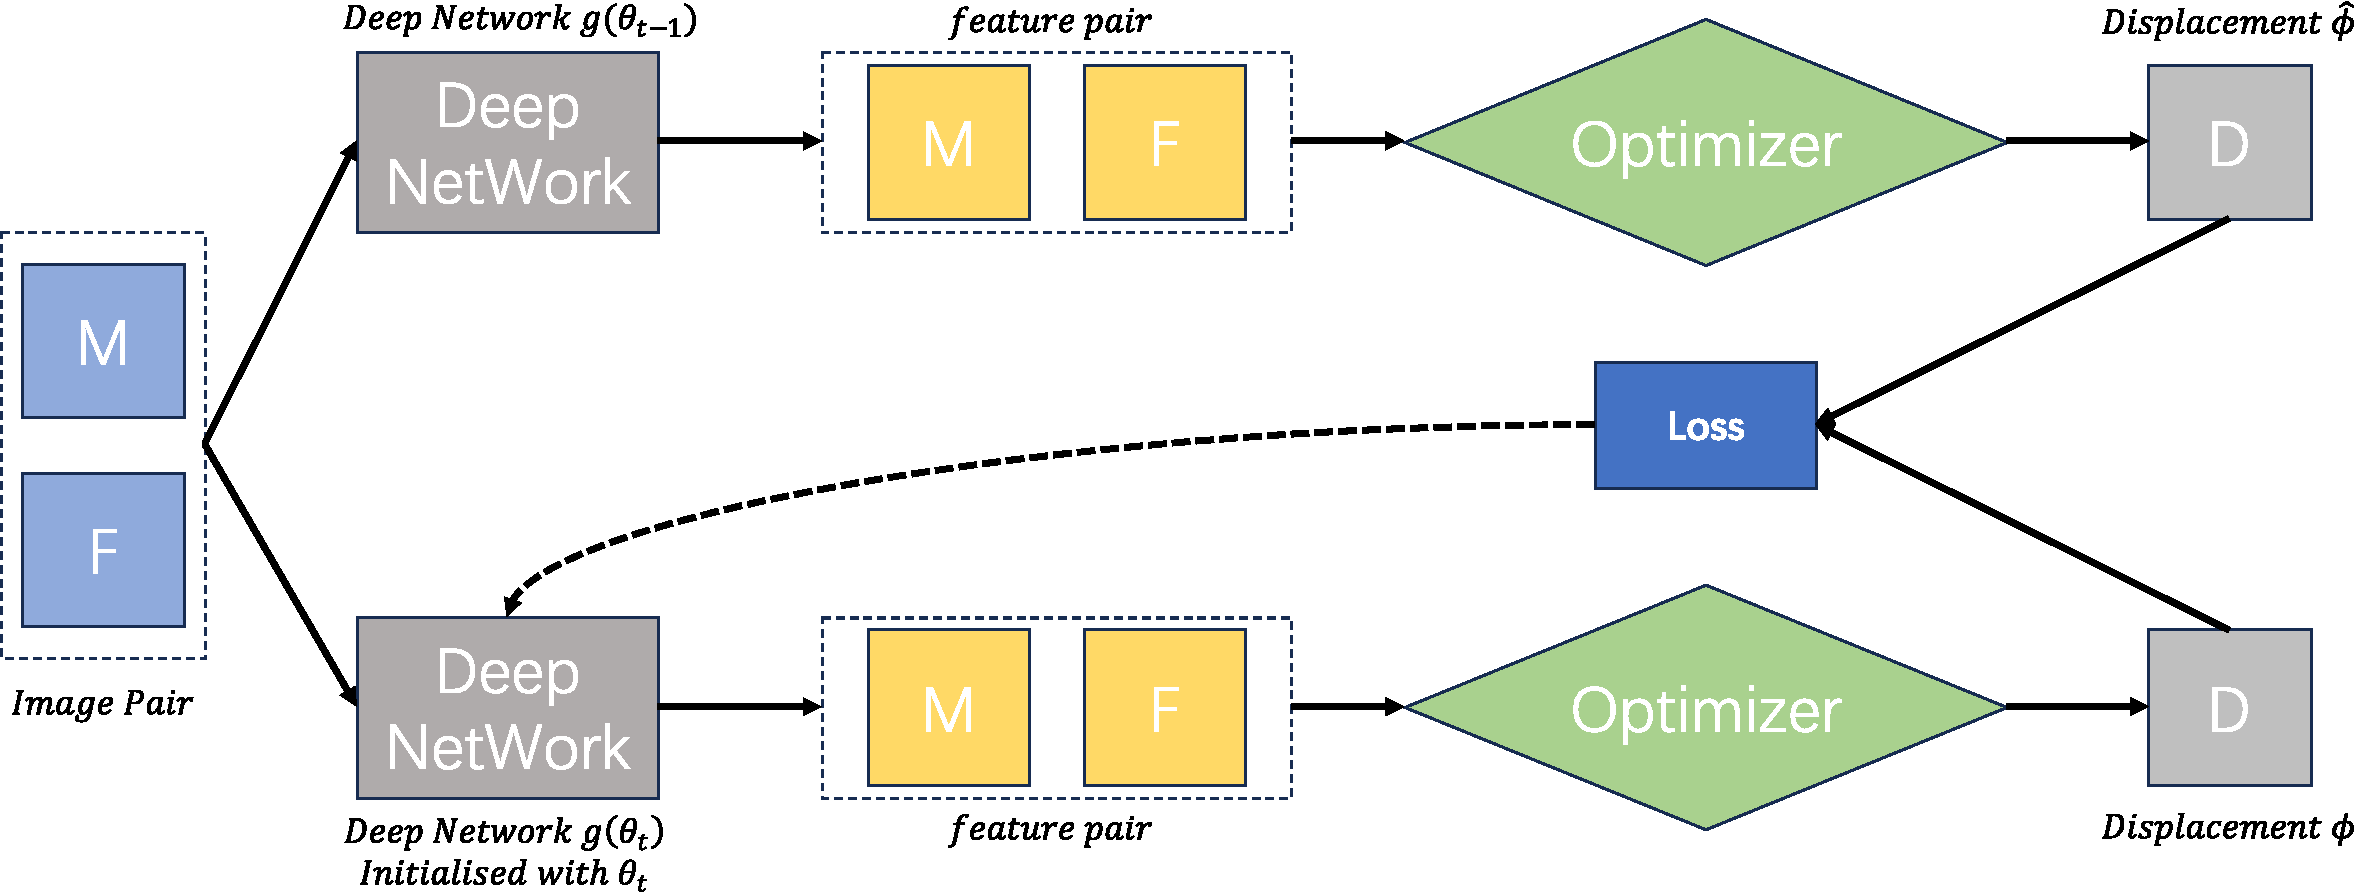
\includegraphics[width=0.9\textwidth]{fig5-cst-crop.pdf}
    \caption{Dice系数随训练epoch的变化曲线}
    \label{fig:regcst}
\end{figure}

对于优化器,采用耦合凸优化器\cite{siebert2022learn},其在给定固定图像和移动图像特征图的情况下,推断出一个位移场,该位移场最小化了平滑度和特征相异度的组合目标。其优化过程包含三个关键步骤:前向-后向一致性约束以减少位移场双向误差、基于变形图像的二次特征对齐以细化局部匹配,以及实例级Adam微调以联合优化特征相似性与正则化项。

\subsection{循环自训练策略}

RegCST的创新性主要体现在其循环自训练机制上。该机制摒弃了传统无监督方法对人工设计相似性度量的依赖,转而通过多阶段交替优化伪标签与网络参数实现自我增强。具体而言,网络初始化阶段利用随机权重特征提取网络生成初始伪位移场,随后通过目标配准误差(TRE)损失函数监督特征网络的训练。每一训练阶段结束后,利用当前网络生成更精确的伪标签,并通过学习率热重启策略跳出局部最优,进入下一轮迭代。针对腹部CT配准任务,该过程通常需经过8个阶段以收敛至最优性能。

RegCST网络采用随机初始参数$\theta_0$初始化特征提取网络来获得用于训练第一个特征提取网络的伪标签监督。

这种设置存在一个关键问题:网络可能会过度拟合初始伪标签,并学习再现的是随机特征。因此,受到对比学习\cite{chen2021exploring}的启发,RegCST网络通过在两个层面上将不对称性纳入学习和伪标签流来提高特征学习的效率。首先,对两个流中的输入对应用不同的随机增广。其次,在优化器之后通过额外微调和正则化步骤来增强伪标签流,以改善伪位移场包括以下三个部分:

\begin{itemize}
    \item 计算反向位移场,然后迭代地最小化两个场之间的差异;这种计算确保了无论数据是朝哪个方向(固定图像到移动图像或反向)进行处理,网络都能够保持一致性,从而提高了最终预测的准确性
    \item 在重复所有先前步骤之前,使用推断的位移场对运动图像进行扭曲;即在实施新的迭代之前,先应用当前的预测到原始运动图像中,以确保生成的伪标签适应最近的网络参数
    \item 通过联合最小化正则化成本和特征相异度,即网络输出特征之间的差异来微调最终位移场;这种优化会减小生成的位移场的复杂性,同时保持与目标的匹配程度,从而改善配准质量
\end{itemize}

自我训练的第一阶段收敛之后,重复该过程$T$次。具体来说,在阶段$t$,使用前一阶段训练的网络$g(\theta_{t-1})$生成精确的伪标签,用$g(\theta_{t-1})$的权重初始化网络$g(\theta_{t})$,并对学习率进行热重启,以避开前一阶段的潜在局部最小值。

\section{本章小结}

本章介绍了MutualReg互学习配准框架的设计及其组成部分,描述了其核心理念和实现过程。MutualReg通过递归学习的方式整合无监督和有监督损失,采用知识蒸馏机制,结合VRC模块,以提高配准精度。首先对MutualReg的框架结构进行了概述,强调了通过相互学习来优化教师和学生网络,并确保通过VRC模块进行可靠的监督信号选择。

接着,介绍了MutualReg框架中所采用的教师网络(PAN网络)和学生网络(RegCST网络)。PAN网络引入了双流金字塔编码器与多头局部注意力Transformer解码器,增强了特征表示能力和形变建模精度。其独特的局部注意力机制通过正交损失解决多头学习的同质性问题,有效地引导学生网络关注最关键的解剖区域。RegCST网络则通过自训练机制和耦合凸优化器,实现了对图像配准的科学精确的应用,逐步提高匹配精度。该网络通过递归自我增强的策略,不断更新生成的伪标签与网络参数,形成闭环优化。

\chapter{基于PAN网络的改进与预训练}

% \section{PAN网络介绍}

% \subsection{PAN网络架构}

% PAN网络是一种用于医学图像配准的无监督深度学习方法,通过结合双流金字塔编码器和多头局部注意力Transformer解码器,有效解决了传统卷积神经网络特征增强不足及Transformer信息冗余的问题。编码器采用通道注意力机制增强多层次特征表示,解码器通过局部注意力Transformer分析运动模式并生成平滑变形场,同时引入正交正则化减少特征冗余以提升运动模式建模能力。其网络架构如图\ref{fig:4}。

% \begin{figure}[h]
%     \centering
%     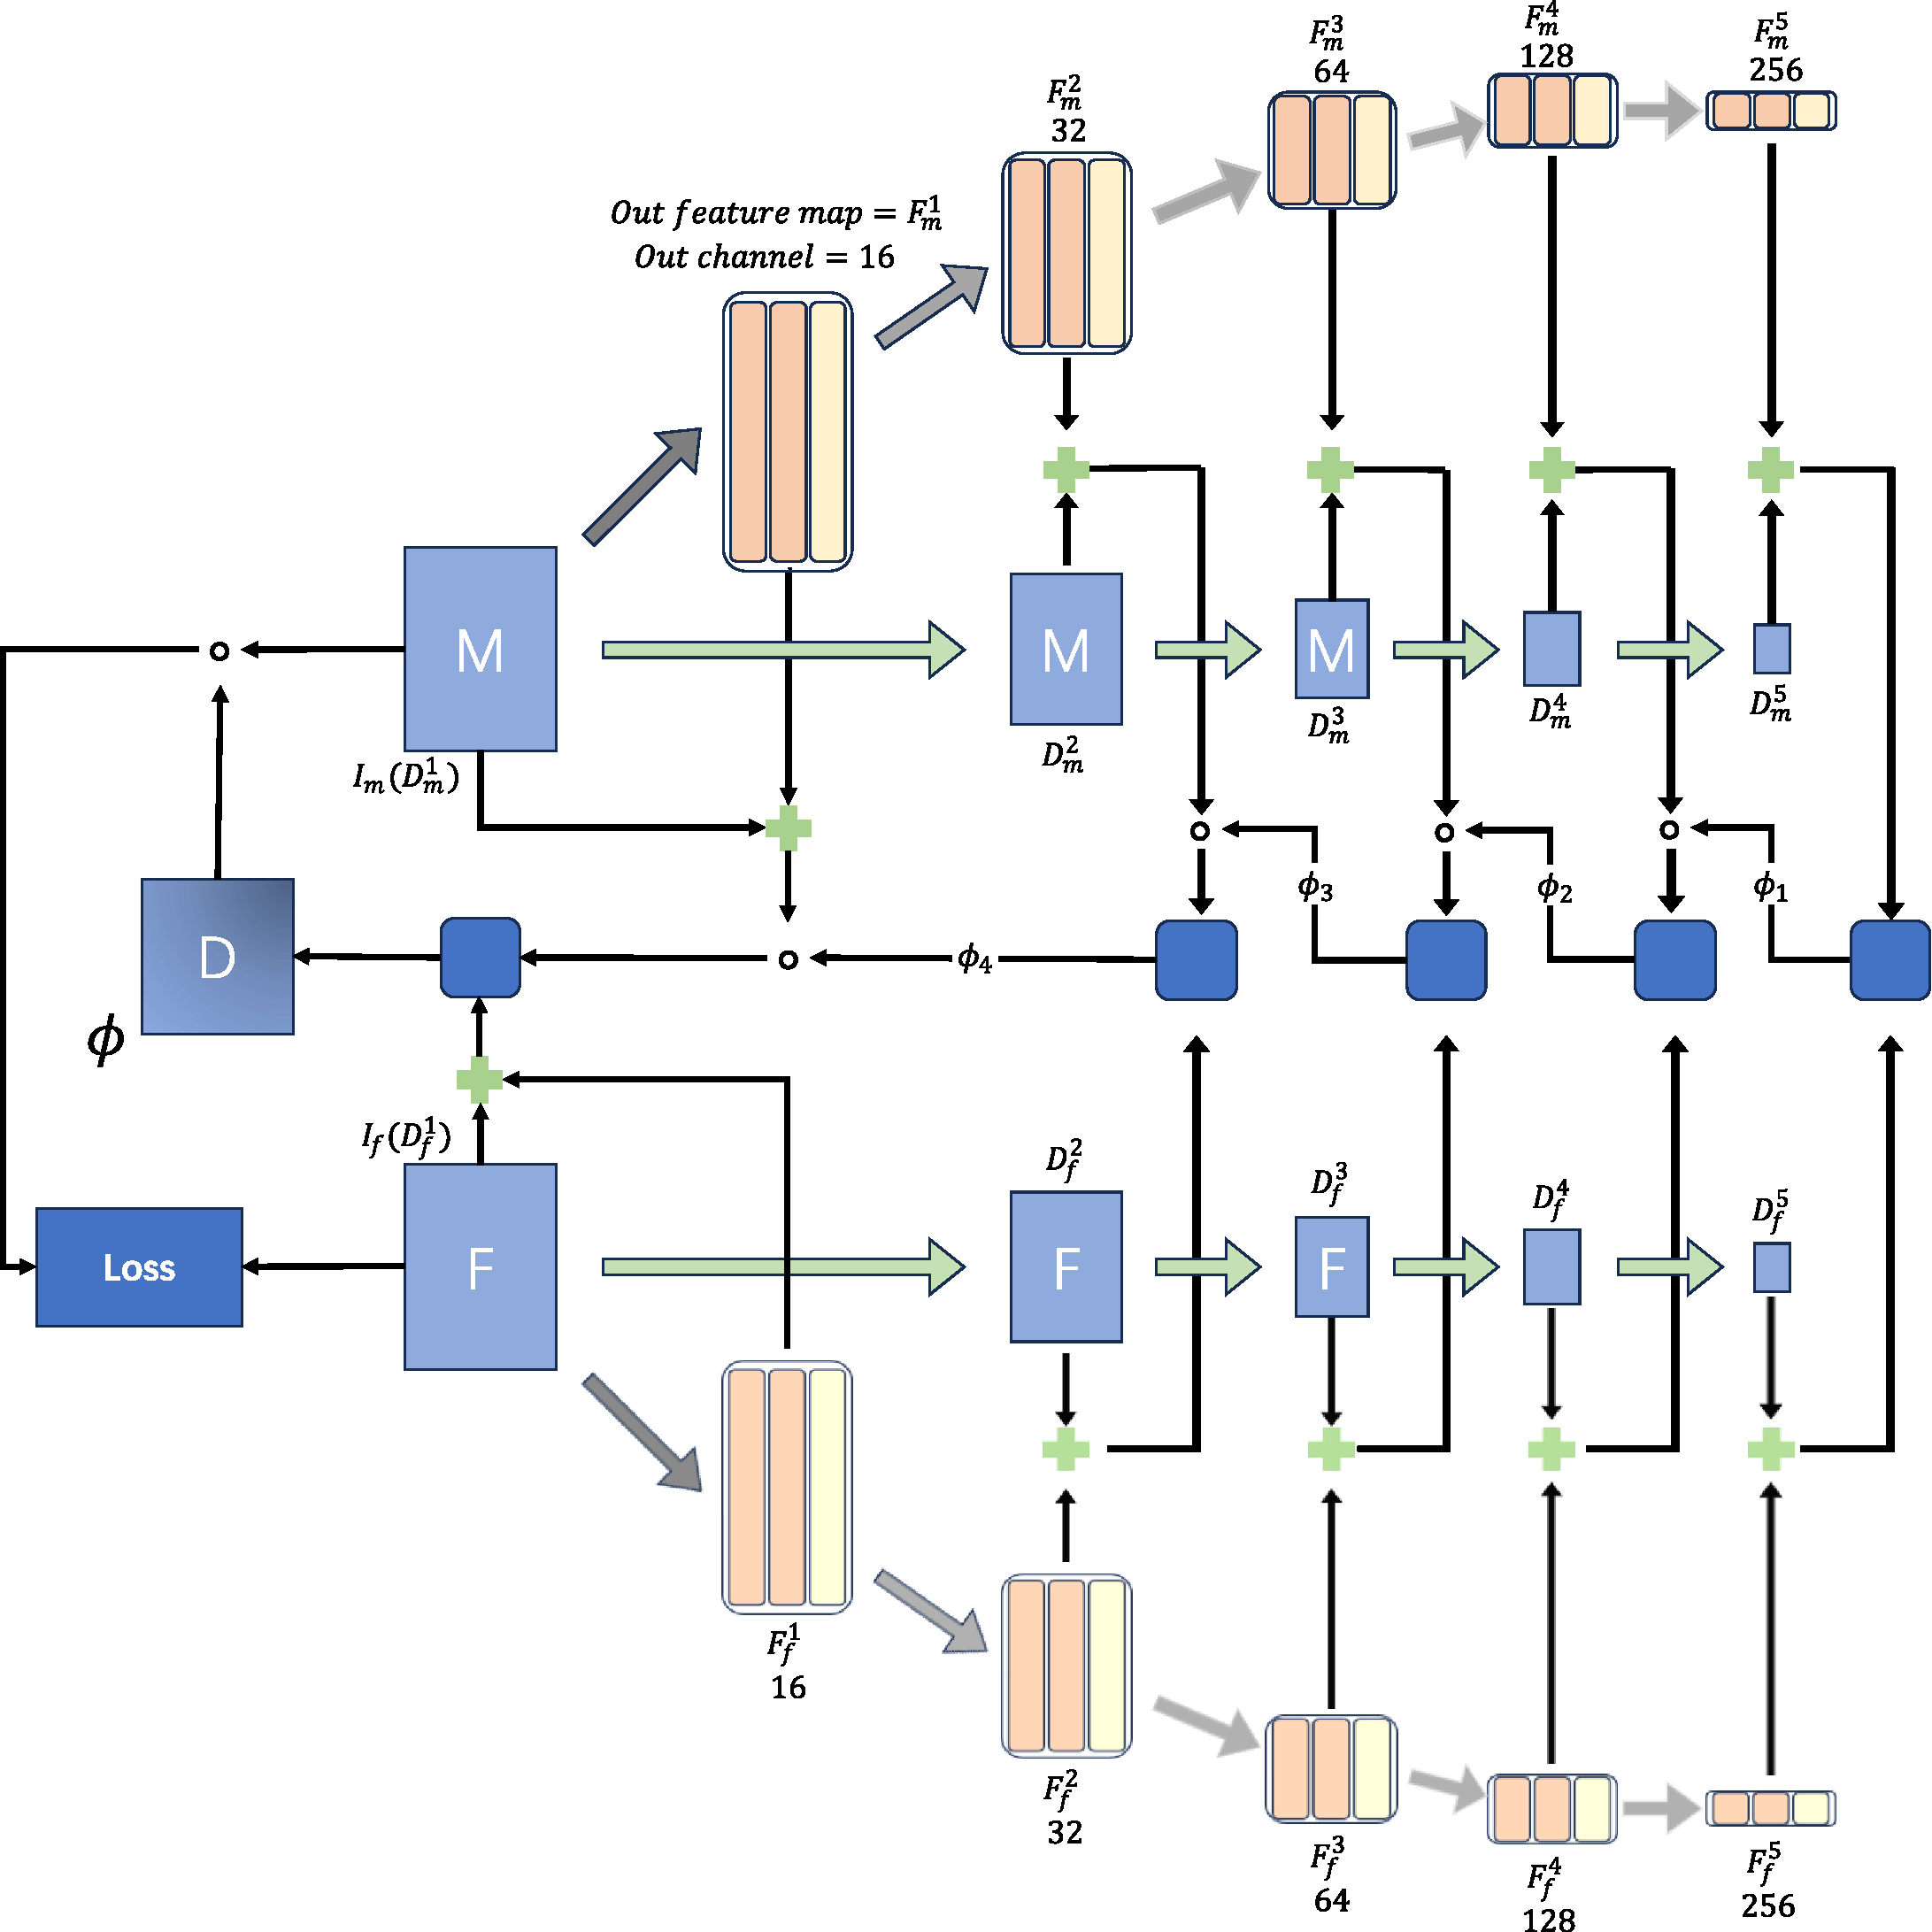
\includegraphics[width=0.7\textwidth]{fig4-PAN-crop.pdf}
%     \caption{PAN网络架构}
%     \label{fig:4}
% \end{figure}

% 其网络主要由双流金字塔编码器和局部注意力Transformer解码器组成。

% 双流权重共享的金字塔编码器使用运动图像$I_m$和固定图像$I_f$作为输入,并通过一系列通道注意力块生成两组分组特征:$\{F_m^1,F_m^2,F_m^3,F_m^4,F_m^5\}$和$\{F_f^1,F_f^2,F_f^3,F_f^4,F_f^5\}$。同时,$I_m$和$I_f$经过下采样生成图像集$\{D_m^1,D_m^2,D_m^3,D_m^4,D_m^5\}$和$\{D_f^1,D_f^2,D_f^3,D_f^4,D_f^5\}$,并于相对对应的特征图进行对齐。

% 对于每个通道注意力块,使用两个卷积块(每个块都有一个$3\times3\times 3$的卷积层、一个实例归一化层\cite{ulyanov2016instance}和一个LeakyReLU激活层)和一个压缩和激励(SE)块\cite{hu2018squeeze}。SE块通过结合全局信息动态优化特征图,促进编码器生成更具代表性的特征。

% 在解码器部分,利用局部注意力Transformer(LAT),来解析特征图并推导出形变场。首先将$(F_m^5,D_m^5)$和$(F_f^5,D_f^5)$输入LAT模块,以分析形变并生成初始形变场$\phi_1$。之后利用$\phi_1$对$(F_m^4,D_m^4)$进行形变,并将$(F_m^4\circ \phi_1,D_m^4\circ\phi_1 )$和$(F_f^4,D_f^4)$做为后续LAT的输入,生成$\phi_2$。类似的,生成$\phi_3,\phi_4$和最终的形变场$\phi$。

% 作为教师网络,PAN网络不仅能引导学生网络识别和关注关键区域,还能通过其强大的特征选择能力,促进学生网络的学习。

% \subsection{局部注意力Transformer模块}

% 局部注意力Transformer模块用于生成每个下采样层的形变场。具体而言将编码器特定层的运动图像特征图、固定图像特征图及其相应的降采样图像分别表示为 \( F_m \)、\( F_f \)、\( D_m \) 和 \( D_f \)。之后,将 \( (F_f, D_f) \) 和 \( (F_m, D_m) \) 在通道维度上进行连接。然后,连接后的特征通过线性投影(LP)和层归一化(LayerNorm,LN)计算查询(Q)和键(K),具体表达如下:

% \begin{equation}
%     Q = LN(LP(\text{concat}(F_f, D_f)))
% \end{equation}

% \begin{equation}
%     K = LN(LP(\text{concat}(F_m, D_m)))
% \end{equation}

% 对于多头注意力机制,\( Q \in \mathbb{R}^{S \times h \times w \times l \times \frac{c}{S}} \) 和 \( K \in \mathbb{R}^{S \times h \times w \times l \times \frac{c}{S}} \) 可以按注意力头的数量 \( S \) 划分为 \( \{ Q_1, Q_2, \ldots, Q_S \} \) 和 \( \{ K_1, K_2, \ldots, K_S \} \),其中 \( c \) 是通道数。那么,第 \( s \) 个注意头的局部注意力图 \( LA \) 可以通过以下公式计算:

% \begin{equation}
%     LA_s = \text{softmax}\left(Q_s \cdot K_s^T + P_s\right)
% \end{equation}

% 其中 \( N(x) \) 表示体素 \( x \) 的 \( N \times N \times N \) 邻域,\( P \in \mathbb{R}^{S \times N \times N} \) 是可学习的相对位置偏差。

% 局部注意力图 \( LA \) 蕴含了不同运动模式的信息。因此,可以利用局部注意力图对规则形变场进行加权,以生成一系列可能的形变子场:

% \begin{equation}
%     \phi_s = LA_s \cdot V
% \end{equation}

% 其中 \( V \in \mathbb{R}^{n \times n \times n} \) 表示邻域质心的相对位置坐标。

% 最后,通过卷积层合并来自每个注意头的形变子场 \( \{ \phi_1, \phi_2, \ldots, \phi_S \} \),以在第 \( t \) 个解码层生成最终的形变场 \( \phi_t \in \mathbb{R}^{h \times w \times l \times 3} \)。

% 在多头学习中会出现潜在同质性问题。潜在同质性可能导致信息冗余,使得多个头部学习到相似的特征,从而降低模型的区分能力和整体性能。这种同质化会导致特征表达不足,影响模型在多类别任务中的判别性,同时也使训练效率降低,浪费计算资源。

% 因此,为了解决多头LAT学习内容的潜在同质性,PAN网络在LAT模块中使用正交损失$L_{orth}$对特征学习进行正则化\cite{brock2016neural}。

% 首先将查询(Q)和键(K)根据注意力头的维度转换为平面向量,形成一个矩阵 \( W \in \mathbb{R}^{S \times u} \)(其中 \( u = h \cdot w \cdot l \cdot c_s \))。在获得矩阵 \( W \) 之后,对每个头部所表示的向量进行归一化处理,并与其转置相乘。最终,正交性损失 \( L_{\text{orth}} \) 可以通过以下公式计算:
% \begin{equation}
%     L_{\text{orth}} = L_{\text{MSE}}\left(\text{Norm}(W) \cdot \text{Norm}(W)^T, I\right)
% \end{equation}

% 其中,\( I \) 是单位矩阵,\( L_{\text{MSE}} \) 是均方误差(即 \( l_2 \) 范数)的计算。

\section{PAN网络与训练数据集适配}

为将PAN网络适配至LUMIR大规模数据集,需重构原始面向LPBA40的数据加载逻辑。本节通过对比分析原始与改进策略,阐述关键适配方法。

原始PAN网络使用LPBA40数据集进行训练,其对于训练图像对的采样采用动态索引映射策略,核心逻辑如算法\ref{alg:alg1-Dynamic Index Generation}。

% \foocaption{\textbf{算法1}: 动态索引生成}
\begin{algorithm}

    \AlgoBiCaption{动态索引生成}{Dynamic Index Generation}\label{alg:alg1-Dynamic Index Generation}
    \KwIn{总图像数 $len$, 当前索引 $index$}
    \KwOut{固定图像序号 $f\_index$, 移动图像序号 $y\_index$}

    $f\_index \gets \lfloor index / (len-1) \rfloor$ \\
    $s \gets index \mod (len-1)$ \\
    \If{$s \geq f\_index$}{
        $y\_index \gets s + 1$
    }
    \Else{
        $y\_index \gets s$
    }
    \Return{$f\_index$, $y\_index$}
\end{algorithm}


该方法的核心特征包括全排列配对、运行时计算和无筛选机制。它通过数学运算生成所有可能的有序对,确保每个样本都与其他所有样本进行配对。同时,该方法在数据加载阶段动态计算配对关系,而不预先存储配对信息。此外,它接受所有可能的配对组合,包括那些在解剖结构上存在显著差异的图像对,从而增强了模型的全面性与适应性。

该策略在LPBA40等小规模数据集(N=40)中是可行的,但在LUMIR(N=3384)场景下却会产生约11.45M个样本对(3384 $\times$ 3383),进而引发一系列问题。首先,训练周期会显著延长,因为单个epoch需处理千万级的样本,使其无法满足实际训练的需求。其次,大量低相似度的配对会导致模型收敛困难,进而影响性能。最后,动态索引计算会增加额外的计算开销,从而加重内存压力,给系统带来负担。

\paragraph{改进适配策略}
针对上述问题,设计如下的三阶段适配框架:

\paragraph{阶段一:配对预计算与存储}


构建离线预处理管道,生成高质量配对信息,如算法\ref{alg:alg2-Similarity-based Image Pairing}。

\begin{algorithm}[h]
    \AlgoBiCaption{基于相似度的图像配对}{Similarity-based Image Pairing}\label{alg:alg2-Similarity-based Image Pairing}
    \KwIn{图像集合 $I$, 相似度矩阵 $S$}
    \KwOut{配对列表 $pairs$}
    初始化 $pairs \gets \emptyset$, $used[i] \gets 0\ \forall i$ \\
    $sorted\_indices \gets \text{argsort}(S, \text{descending=True})$ \\
    \For{$(i,j) \in sorted\_indices$}{
    \If{$i == j$}{
        \Continue % 使用定义好的 \Continue
    }
    \If{$used[i] < 2$ \textbf{and} $used[j] < 2$}{
        $pairs.\text{append}((i,j))$ \\
        $used[i] \gets used[i] + 1$ \\
        $used[j] \gets used[j] + 1$
        }
        \If{$\min(used) > 0$}{
            \Break % 使用定义好的 \Break
        }
    }
    保存 $pairs$ 至 JSON \\
    \Return{$pairs$}
\end{algorithm}

该算法通过优先选择高MSE相似度的配对,并施加配对次数约束,在保证数据质量的同时控制训练规模。表\ref{tab1}对比了改进前后的核心差异。

\begin{table}[!h]
    \centering
    \caption{原始与改进采样策略对比}
    \label{tab1}
    \begin{tabular}{lll}
        \toprule
        \textbf{特征} & \textbf{原始策略(LPBA40)} & \textbf{改进策略(LUMIR)} \\
        \midrule
        配对生成方式      & 动态全排列                 & 预计算相似度筛选             \\
        配对数量        & $N \times (N-1)$      & 可控(本文1835对)          \\
        存储形式        & 无持久化存储                & JSON文件存储             \\
        数据质量保证      & 无                     & MSE阈值筛选              \\
        扩展性         & 小规模数据集                & 大规模数据集               \\
        \bottomrule
    \end{tabular}
\end{table}



\paragraph{阶段二:数据集类重构}
设计LUMIRDataset类实现高效数据加载,如算法\ref{alg:alg3-Data Loading and Preprocessing}。

\begin{algorithm}

    \AlgoBiCaption{数据加载与预处理}{Data Loading and Preprocessing}\label{alg:alg3-Data Loading and Preprocessing}
    \KwIn{JSON文件路径 $json\_path$}
    \KwOut{标准化图像对 $(I_i, I_j)$}

    加载 $paths$ 和 $pairs$ 从 JSON \\
    实现 \texttt{\_\_getitem\_\_}(index): \\
    \Indp
    $(i,j) \gets pairs[index]$ \\
    $I_i \gets \text{加载图像}(paths[i])$ \\
    $I_j \gets \text{加载图像}(paths[j])$ \\
    $I_i \gets \text{N4矫正}(I_i)$; $I_j \gets \text{N4矫正}(I_j)$ \\
    $I_i \gets \text{Z-score标准化}(I_i)$; $I_j \gets \text{Z-score标准化}(I_j)$ \\
    \Return{$(I_i, I_j)$}

\end{algorithm}

改进点包括:静态配对访问、路径映射优化和批量预处理。首先,通过直接读取预先存储的配对索引,消除了动态计算带来的开销。其次,引入JSON文件实现图像路径到内存索引的快速映射,有效提升了访问效率。最后,在数据加载前完成强度归一化等必要的操作,使得批量预处理能够提高数据准备的效率,从而加快整体训练过程。



\paragraph{阶段三:训练流程整合}
在训练器中集成新的数据加载逻辑,如算法\ref{alg:alg4-Model Training Pipeline}。
\begin{algorithm}

    \AlgoBiCaption{模型训练流程}{Model Training Pipeline}
    \label{alg:alg4-Model Training Pipeline}
    \KwIn{训练轮次 $epochs$, 批次大小 $batch\_size$}
    \KwOut{训练完成的模型 $model$}

    离线生成 $pairs.json$ \\
    初始化 $dataset \gets \text{CustomDataset}(pairs.json)$ \\
    初始化 $dataloader \gets \text{DataLoader}(dataset, batch\_size)$ \\
    \For{$epoch \gets 1$ \KwTo $epochs$}{
        \For{$(batch\_x, batch\_y) \in dataloader$}{
            前向传播与损失计算 \\
            反向传播更新参数
        }
    }
    \Return{$model$}
\end{algorithm}


\section{损失函数改进}

在原始PAN网络中,损失函数采用三任务联合优化框架,,用于提升模型的图像配准质量、多头注意力机制效率以及位移场的平滑性,如公式(\ref{eq:1}):

\begin{equation}
    \mathcal{L}_{\text{total}} = \underbrace{\lambda_1 \mathcal{L}_{\text{NCC}}}_{\text{图像相似度}} + \underbrace{\lambda_2 \mathcal{L}_{\text{Ortho}}}_{\text{注意力正则}} + \underbrace{\lambda_3 \mathcal{L}_{\text{Reg}}}_{\text{位移场平滑}}
    \label{eq:1}
\end{equation}

具体而言,损失函数的各个部分如下:

\begin{itemize}
    \item \textbf{图像相似度损失}:衡量配准图像与目标图像的局部相关性,原始PAN网络使用NCC指标进行衡量

    \item \textbf{多头注意力正交损失}:约束多头注意力权重的正交性
          \begin{equation}
              \mathcal{L}_{\text{Ortho}} = \sum_{l=1}^L \|W_l^T W_l - I\|_F^2
          \end{equation}
          $W_l$为第$l$层注意力头的权重矩阵

    \item \textbf{位移场正则损失}:采用三阶Bending Energy约束形变场平滑性
          \begin{equation}
              \mathcal{L}_{\text{Reg}} = \int_\Omega \|\nabla^3 \phi\|^2 dx
          \end{equation}
\end{itemize}

其中$\lambda_1$、$\lambda_2$、$\lambda_3$为权重系数。

通过这样的损失函数设计,PAN网络能够在保证图像配准质量的前提下,提升多头注意力机制的效率,并确保位移场的平滑性。


在进行训练时,为了保证模型在大数据集下的收敛性以及泛化能力,同时为了提高模型对同图像域中空间特征变化的鲁棒性,新损失函数在保持正交约束的基础上对图像相似性损失和位移场平滑正则损失进行改进,改进后的联合损失函数如公式(\ref{eq:2}):

\begin{equation}
    \mathcal{L}_{\text{new}} = \underbrace{\mu_1 \mathcal{L}_{\text{MIND}}}_{\text{跨模态相似度}} + \underbrace{\mu_2 \mathcal{L}_{\text{Ortho}}}_{\text{注意力正则}} + \underbrace{\mu_3 \mathcal{L}_{\text{smh}}}_{\text{位移场平滑}}
    \label{eq:2}
\end{equation}

\begin{itemize}
    \item \textbf{MIND损失}:基于模态无关局部描述符的相似性度量,对强度分布变化具有鲁棒性

    \item \textbf{位移场平滑度正则化损失}:位移场空间梯度上的扩散正则化
          \begin{equation}
              L_{smh}(\phi)=\frac{1}{|\Omega|}\sum_{v\in\Omega}|\nabla \phi(v)
          \end{equation}

\end{itemize}

其中$\nabla \phi(v)$表示体素$v$处位移场$\phi$的梯度,$\mu_1$、$\mu_2$、$\mu_3$为权重系数。

在新的损失函数设计中,PAN网络得到了改进,以适应大数据集的训练需求和增强模型的泛化能力及鲁棒性。这些变化通过三个方面的优化得以实现:图像相似性度量的改进、注意力机制的保持以及位移场正则化方法的改变。

首先,新的损失函数使用MIND(Modality Independent Neighbourhood Descriptor)损失来替代原始的NCC损失。这一变化的优势在于MIND损失能够更好地处理跨模态图像间的配准问题。传统的NCC主要适用于单模态配准,对不同模态间的强度差异较为敏感,而MIND损失则基于模态无关局部描述符进行相似性度量,能够更具鲁棒性地捕捉到复杂场景下跨模态图像间的相似性,从而提高图像配准质量。

其次,尽管新损失函数在某些方面进行了改进,它仍然保持了对多头注意力正交约束的重视。这一点确保了注意力机制在特征提取过程中的有效性,促进了不同注意力头之间的独立性以及模型的表达能力。通过正交约束,多头注意力模块能够更有效地提取多样化的特征,这对改善模型整体性能至关重要。

最后,新损失函数引入了基于位移场空间梯度上的扩散正则化损失来替换原有的位移场正则化。这一变更通过对形变场的同胚性质进行惩罚和正则化,增强了位移场在变形过程中的合理性和光滑性。确保生成的形变场不出现局部折叠和不连续性,从而进一步提高模型的稳定性和可靠性。

这些改进不仅强化了PAN网络的训练稳定性,还增强了其在不同配准任务中的适应能力。整体而言,新损失函数的设计使模型在处理多模态数据和不同场景下的空间特征变化时,能够获得更好的收敛性和泛化性能。

\section{实验过程与结果分析}

训练中,使用预先使用N4校正和Z-Score归一化并经过相似性阈值筛选后的LUMIR数据集进行训练,联合损失函数中的各个损失函数权重都设置为1,使用Adam优化器。Adam优化器学习率设置为0.0001,使用AMSGrad 变体,L2正则参数设置为0。模型的训练周期设置为50轮,每轮batch为1。训练过程中使用的团硬件配置参数如表\ref{tab:environment}。

\begin{table}[ht]
    \centering
    \caption{软硬件参数表}
    \begin{tabular}{c c}
        \toprule
        \textbf{项目} & \textbf{内容}                 \\
        \midrule
        GPU         & NVIDIA P40 GPU (24GB显存) * 1 \\
        CPU         & Intel Xeon E5-2686 v4 CPU   \\
        内存          & 31GB                        \\
        CUDA        & 12.1                        \\
        操作系统        & Linux                       \\
        深度学习框架      & PyTorch 2.2.1               \\
        \bottomrule
    \end{tabular}
    \label{tab:environment}
\end{table}

经过训练的模型在LPBA40数据集上进行评价,每轮次训练完成后使用Dice指标对模型配准精度进行评价。Dice系数随训练轮次增加的变化图像如图\ref{fig:PANDice}。

关键发现显示模型在收敛特性和稳定性方面的显著改进。首先,如图\ref{fig:PANDice}所示,Dice系数在前10个epoch中从54.1\%迅速升至65.2\%,这表明MIND损失在初期收敛方面发挥了积极作用。其次,经过损失函数的改进,模型在训练结束时的性能指标波动维持在1.2\%以内,从而有效避免了模型收敛困难的情况。这些发现共同指向了新损失函数对于提升模型训练质量的重要性。

\begin{figure}[h]
    \centering
    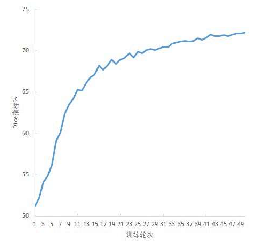
\includegraphics[width=0.7\textwidth]{PAN-crop.pdf}
    \caption{Dice系数随训练epoch的变化曲线}
    \label{fig:PANDice}
\end{figure}

整体训练完成后,选择最优模型在LPBA40数据集上进行评价。具体而言,从两个方面进行评价:用Dice系数衡量的配准精度以及用SDlogJ指标衡量的位移场平滑性。由于PAN网络原始模型在衡量生成位移场平滑性时并未使用SDlogJ指标进行评价,而是使用的|J(φ)|<0的占比进行评价。因此为了使得两个网络更具对比性,增加改进模型使用|J(φ)|<0占比的评价结果。预训练完成后模型的性能评价以及与原始网络的对比如表\ref{tab:PANresult}。

\begin{table}[h]
    \centering
    \caption{模型性能定量对比}
    \label{tab:PANresult}
    \begin{tabular}{lcc}
        \toprule
        \textbf{指标} & \textbf{原始模型} & \textbf{改进模型} \\
        \midrule
        Dice系数      & 71.1\%        & 72.2\%        \\
        SDlogJ      & -             & 0.151         \\
        |J(φ)|<0    & 0.0001\%      & 0.0001\%      \\
        \bottomrule
    \end{tabular}
\end{table}

在对改进后的PAN网络模型进行训练与评估后,结果表明该模型在LPBA40数据集上表现出色。首先,Dice系数的显著提升,从71.1\%提高到72.2\%,说明新设计的损失函数有效增强了模型在图像配准中的准确性。此外,训练过程中模型的收敛速度也明显加快,特别是在前10个epoch内,Dice系数迅速提高,表明改进的损失函数特别适合促进初期收敛。

在稳定性方面,训练末期的指标波动控制在1.2\%以内,显示出改进模型在收敛后保持性能一致性方面的优势。这种稳定性将有助于在实际应用中减少不确定性,从而增强模型的实用性。

最后,位移场的平滑性评估也显示出改进效果,其中使用SDlogJ指标得到了0.151的结果,以及|J(φ)|<0的折叠点比例为0.0003\%,进一步表明模型在生成合理变形场方面的能力。


\section{本章小结}

本章围绕PAN网络在大规模医学图像配准任务中的适配与优化展开研究。首先,针对LUMIR数据集3384张图像的全排列配对产生1145万对样本导致的训练效率问题,采用基于MSE相似度的预计算配对策略,通过离线筛选生成1835对高相似度图像。接着,在数据加载流程中重构数据集类,建立JSON索引映射机制,实现静态配对访问与批量预处理。然后,在损失函数方面,将原始NCC相似性度量替换为模态无关的MIND描述符,并在位移场正则化中采用梯度扩散约束替代Bending Energy,改进后模型在LPBA40测试集上的Dice系数达到72.2\%,较原始模型提升1.1个百分点。最后,实验数据显示,前10个训练epoch内Dice系数从54.1\%快速上升至65.2\%。位移场平滑性指标SDlogJ为0.151,折叠点占比(|J(φ)|<0)稳定在0.0003\%以下。训练过程中采用固定权重系数(μ₁=μ₂=μ₃=1),模型在50个epoch内的性能波动幅度控制在1.2\%以内。

\chapter{基于RegCST网络的改进与预训练}

% \section{RegCST网络介绍}

% \subsection{RegCST网络架构}

% RegCST是一种基于循环自训练策略的无监督3D医学图像配准框架,其核心架构通过深度融合深度特征提取网络与可微分优化算法,实现了从伪标签生成到网络参数更新的闭环优化。如图\ref{fig:regcst}所示,该网络主要由特征提取模块、优化器模块及自训练机制三部分构成。特征提取模块采用标准3D卷积神经网络,包含6层卷积操作,每层卷积核尺寸为$3 \times 3 \times 3$,通道数逐层递增(32、64、128),并通过步长为2的下采样将输入图像分辨率缩减至原始尺寸的1/8。网络末端通过$1 \times 1 \times 1$卷积将固定图像与移动图像的特征映射至16维空间,并输入相关性层计算多尺度位移匹配响应,为后续优化提供高判别性特征表示。

% \begin{figure}[h]
%     \centering
%     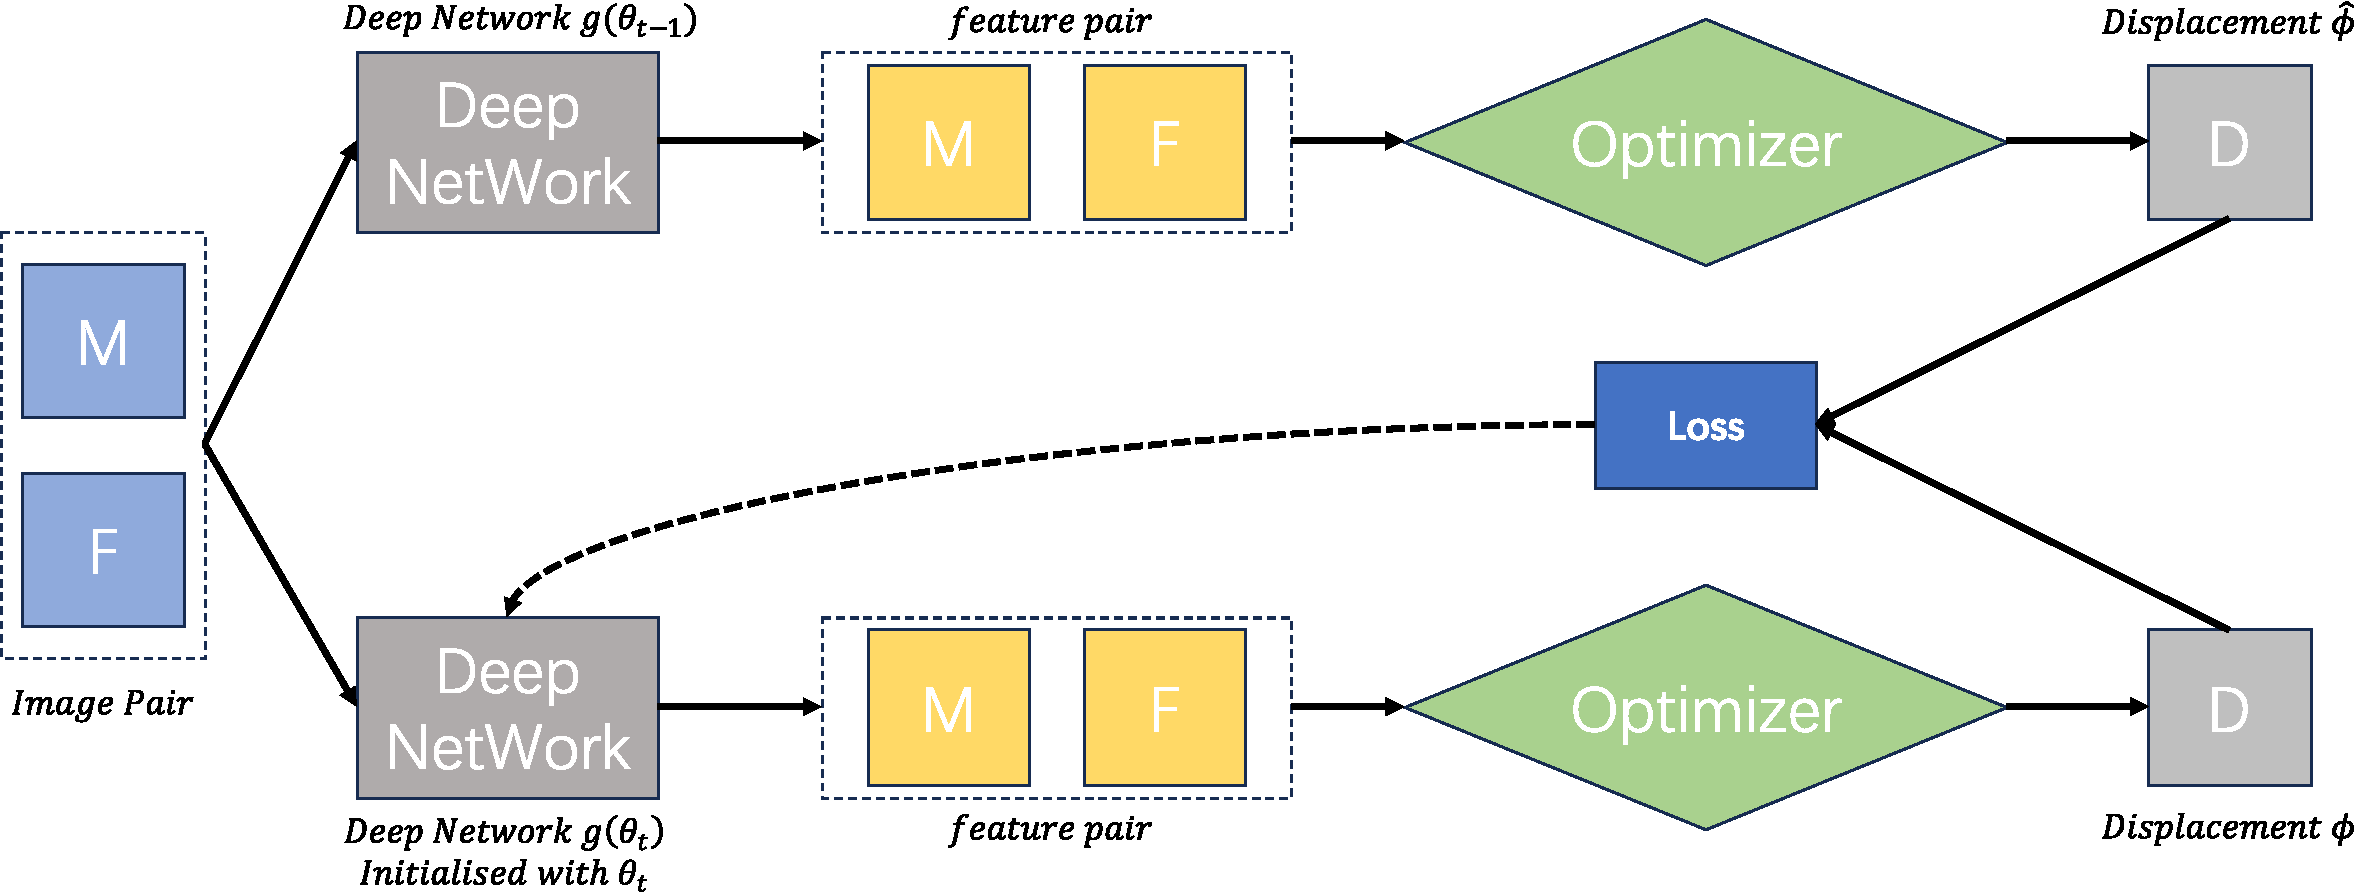
\includegraphics[width=0.7\textwidth]{fig5-cst-crop.pdf}
%     \caption{Dice系数随训练epoch的变化曲线}
%     \label{fig:regcst}
% \end{figure}

% 对于优化器,采用耦合凸优化器\cite{siebert2022learn},其在给定固定图像和移动图像特征图的情况下,推断出一个位移场,该位移场最小化了平滑度和特征相异度的组合目标。其优化过程包含三个关键步骤:前向-后向一致性约束以减少位移场双向误差、基于变形图像的二次特征对齐以细化局部匹配,以及实例级Adam微调以联合优化特征相似性与正则化项。

% \subsection{循环自训练策略}

% RegCST的创新性主要体现在其循环自训练机制上。该机制摒弃了传统无监督方法对人工设计相似性度量的依赖,转而通过多阶段交替优化伪标签与网络参数实现自我增强。具体而言,网络初始化阶段利用随机权重特征提取网络生成初始伪位移场,随后通过目标配准误差(TRE)损失函数监督特征网络的训练。每一训练阶段结束后,利用当前网络生成更精确的伪标签,并通过学习率热重启策略跳出局部最优,进入下一轮迭代。针对腹部CT配准任务,该过程通常需经过8个阶段以收敛至最优性能。

% RegCST网络采用随机初始参数$\theta_0$初始化特征提取网络来获得用于训练第一个特征提取网络的伪标签监督。

% 这种设置存在一个关键问题:网络可能会过度拟合初始伪标签,并学习再现的是随机特征。因此,受到对比学习\cite{chen2021exploring}的启发,RegCST网络通过在两个层面上将不对称性纳入学习和伪标签流来提高特征学习的效率。首先,对两个流中的输入对应用不同的随机增广。其次,在优化器之后通过额外微调和正则化步骤来增强伪标签流,以改善伪位移场包括以下三个部分:

% \begin{itemize}
%     \item 计算反向位移场,然后迭代地最小化两个场之间的差异;这种计算确保了无论数据是朝哪个方向(固定图像到移动图像或反向)进行处理,网络都能够保持一致性,从而提高了最终预测的准确性
%     \item 在重复所有先前步骤之前,使用推断的位移场对运动图像进行扭曲;即在实施新的迭代之前,先应用当前的预测到原始运动图像中,以确保生成的伪标签适应最近的网络参数
%     \item 通过联合最小化正则化成本和特征相异度,即网络输出特征之间的差异来微调最终位移场;这种优化会减小生成的位移场的复杂性,同时保持与目标的匹配程度,从而改善配准质量
% \end{itemize}

% 自我训练的第一阶段收敛之后,重复该过程$T$次。具体来说,在阶段$t$,使用前一阶段训练的网络$g(\theta_{t-1})$生成精确的伪标签,用$g(\theta_{t-1})$的权重初始化网络$g(\theta_{t})$,并对学习率进行热重启,以避开前一阶段的潜在局部最小值。


\section{RegCST网络与训练数据集适配}

原始RegCST网络针对小规模数据集设计了全内存驻留的训练范式,其核心策略在于将全部20对训练数据一次性载入GPU显存,并通过动态权重采样机制优化训练过程。该权重采样的实现依托于两轮优化框架:首先通过凸优化算法生成初始形变场$\phi_0$,随后采用Adam优化器对其进行微调得到$\phi_{\text{finetune}}$,最终以形变场差异$\|\phi_{\text{finetune}} - \phi_0\|_2$作为采样权重,差异越大的图像对获得更高的训练优先级。这种设计在小规模场景下可有效聚焦于困难样本,但面对本研究涉及的1835对训练数据时,仅存储原始图像就需要约50GB显存,若进一步缓存形变场中间状态将远超P40显卡的24GB显存容量,存在严重的内存墙限制。

\begin{algorithm}[h]
    \AlgoBiCaption{数据分块与批次加载}{Data Block Partition and Loading}\label{alg:datablock}
    \KwIn{原始图像集合 $I$, 相似度矩阵 $S \in \mathbb{R}^{N \times N}$}
    \KwOut{分块列表 $blocks$}
    初始化 $pairs \gets$ 基于$S$的相似度排序配对结果(算法\ref{alg:alg2-Similarity-based Image Pairing}) \\
    $sorted\_pairs \gets \text{按配对相似度降序排列}(pairs)$ \\
    将$sorted\_pairs$划分为$K$个子集$\{B_1,B_2,...,B_K\}$,其中$|B_i|=100$($i<K$),$|B_K|=35$ \\
    \ForEach{块 $B_i \in \{B_1,...,B_K\}$}{
        加载$B_i$对应的图像对至GPU显存 \\
        初始化块内采样权重$w_j \gets 1.0\ \forall (I_m^j,I_f^j) \in B_i$ \\
        $blocks.\text{append}(B_i)$
    }
    \Return{$blocks$}
    \label{alg:c-regcst-1}
\end{algorithm}

因为在训练时RegCST网络需要根据全部图像对之间的位移场信息来保证权重采样机制的有效性,因此将全部数据分batch进行训练的方法具有一定的局限性。因此受到渐进式课程学习的启发,采用分批次循环训练的方式以应对上述问题。根据实际测试,在24G显存的P40GPU上,单批次最大可承载100对图像训练。因此将全体训练数据划分为19个数据批次(前18批次各含100对,最后一批含35对),如算法\ref{alg:c-regcst-1}。同时在划分数据时,使用MSE指标来衡量图像对之间的相似性,相似性越大的图像对越早被模型训练。训练流程采用分阶段递进策略:加载首个高相似度数据批次后,进行8轮循环自训练,期间动态更新该块内各图像对的采样权重;完成当前块训练后释放显存资源,载入下一数据块重复上述过程,直至遍历全部19个数据块,如算法\ref{alg:c-cst-2}。这种设计融合了课程学习的思想,通过渐进式增加数据复杂度的方式降低模型初期优化难度,同时分块机制将峰值显存占用控制在21.3GB以内。

\begin{algorithm}[h]
    \AlgoBiCaption{分块循环自训练}{Block-wise Cyclic Self-Training}\label{alg:block_training}
    \KwIn{分块数据$blocks$, 初始模型参数$\theta_0$, 最大训练轮次$E=8$}
    \KwOut{优化后模型参数$\theta$}
    \ForEach{块 $B_i \in blocks$}{
        加载$B_i$至GPU显存 \\
        初始化$\theta \gets \theta_0$ \\
        \For{$epoch \gets 1$ \textbf{to} $E$}{
            根据采样权重$w_j$对$B_i$进行加权批次采样 \\
            \ForEach{批次 $(I_m^j,I_f^j) \in B_i$}{
                前向传播生成初始位移场$\phi_0^j \gets f_\theta(I_m^j,I_f^j)$ \\
                凸优化生成伪标签$\phi_{pseudo}^j \gets \text{Optimizer}(I_m^j,I_f^j)$ \\
                Adam微调$\phi_{finetune}^j \gets \text{Adam}(\phi_0^j, \phi_{pseudo}^j)$ \\
                计算位移差异$d_j \gets \|\phi_{finetune}^j - \phi_0^j\|_2$ \\
                更新采样权重$w_j \gets d_j / \sum_k d_k$
            }
            更新模型参数$\theta \gets \text{Adam}(\theta, \nabla_\theta L)$
        }
        释放当前块显存 \\
        保存$\theta$作为下一块初始参数
    }
    \Return{最终模型参数$\theta$}
    \label{alg:c-cst-2}
\end{algorithm}


\section{损失函数改进}

原始RegCST网络的训练范式建立在逐阶段伪标签自监督框架之上,其损失函数设计完全依赖于前一阶段网络输出的位移场监督信号。其原始损失函数为:

\begin{equation}
    \mathcal{L}_{un}^{CST}=TRE(h(g(I_f,I_m;\theta_t)),h(g(I_f,I_m;\theta_{t-1})))
    \label{eq:3}
\end{equation}

其中,$TRE$为两个网络输出的位移场间逐元素目标配准误差的平均值;$g(I_f,I_m;\theta_t)$表示在参数$\theta_t$下特征提取网络提取到的运动图像和固定图像的特征值,$h(g(I_f,I_m;\theta_t))$表示优化器根据特征提取网络输出的特征图进行迭代优化输出的位移场。

在每轮循环自训练中,网络通过8轮迭代(每轮1000次参数更新)逐步优化$\theta_t$,并在每轮结束后将$\phi_t$作为新的监督信号。这一设计的核心假设是迭代优化过程中位移场的渐进式改进,但其潜在风险在于初始阶段的监督信号$\phi_0$由随机初始化网络生成,本质上是对噪声的拟合。实验表明,当初始伪标签质量较低时,网络可能陷入“自证循环”(self-justifying loop),即后续阶段的学习目标退化为对随机噪声模式的复现,而非真实的解剖结构对齐规律。

为了应对这一潜在风险,在具体的训练过程中,对损失函数进行改进。在保留位移场相似性约束的同时,引入模态无关的图像相似性度量作为联合优化目标。这一改进的合理性源于多任务学习的视角:位移场一致性损失确保形变参数的平滑过渡,避免训练过程的剧烈震荡;而MIND损失则从图像内容层面提供跨模态的语义对齐指引。二者的协同作用在初始训练阶段尤为重要,当伪标签$\phi_{t-1}$因网络未充分训练而包含较大误差时,MIND损失可提供独立于网络当前状态的稳定监督信号,有效抑制错误传播。改进后的损失函数定义为:

\begin{equation}
    \mathcal{L}_{\text{new}} = \lambda_1 \underbrace{TRE(h(g(I_f,I_m;\theta_t)),h(g(I_f,I_m;\theta_{t-1})))}_{\text{位移场一致性}} + \lambda_2 \underbrace{\mathcal{L}_{MIND}(I_f,I_m\circ \phi)}_{\text{图像相似性}}
\end{equation}

其中$\mathcal{L}_{MIND}$表示模态无关邻域描述符描述的图像相似性损失。$\lambda_1$和$\lambda_2$为权重系数。



\section{实验过程与结果分析}

训练中,使用预先使用 N4 校正和 Z-Score 归一化并经过相似性阈值筛选后的LUMIR 数据集进行训练,联合损失函数中各个损失函数权重采用动态调整的策略,在前4批数据进行训练时,相似性损失占据主导地位其权重设置为2,位移场一致性损失权重设置为1。在后续训练过程中,则更加注重网络自监督带来的训练效果,相似性损失设置为1,位移场一致性损失设置为2。模型在每批次数据上完成8轮自循环训练,每轮自循环训练共1000次迭代。软硬件参数与PAN网络预训练相同。

\begin{figure}[h]
    \centering
    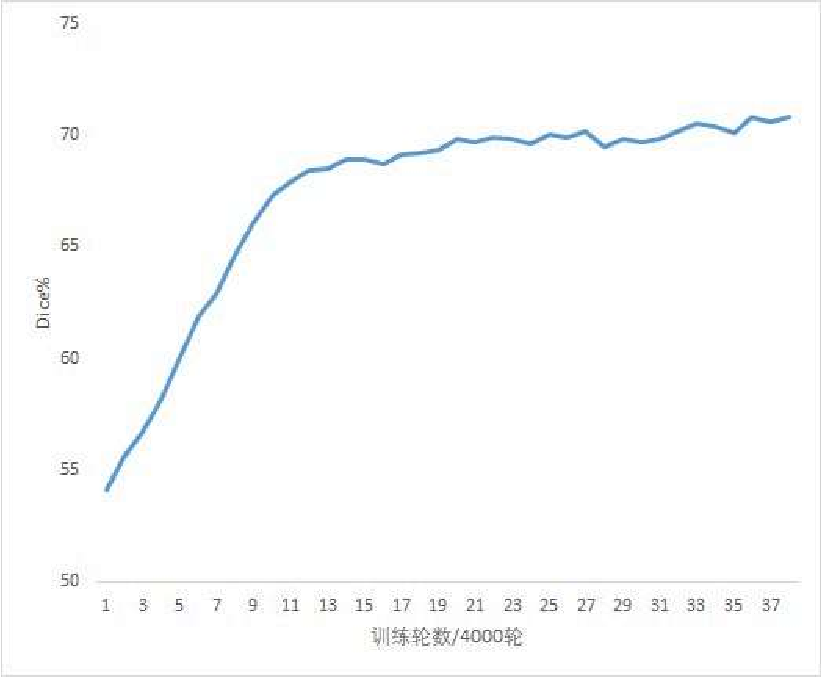
\includegraphics[width=0.7\textwidth]{cst-crop.pdf}
    \caption{Dice系数随训练epoch的变化曲线}
    \label{fig:cstloss}
\end{figure}

经过训练的模型在LPBA40数据集上进行评价,每4000次迭代后使用Dice指标对模型性能进行评价。Dice系数随训练过程的变化图像如图\ref{fig:cstloss}。


如图\ref{fig:cstloss},模型在收敛特性方面有明显改进。Dice系数在前10个epoch中从54.2\%上升至67.3\%。这表明MIND损失在训练初期发挥了积极作用,能够促进模型性能的提升,并且避免学习随机特征的风险。这也能表明新损失函数对于模型训练效果提升的重要性。

整体训练完成后,选择最优模型在 LPBA40 数据集上进行评价。具体而言,从两个方面进行评价:用 Dice 系数衡量的配准精度以及用 SDlogJ 指标衡量的位移场平滑性。具体的对比指标如表\ref{tab:CSTresult}。

\begin{table}[h]
    \centering
    \caption{模型性能定量对比}
    \label{tab:CSTresult}
    \begin{tabular}{lcc}
        \toprule
        \textbf{指标} & \textbf{原始模型} & \textbf{改进模型} \\
        \midrule
        Dice系数      & 69.8\%        & 70.6\%        \\
        SDlogJ      & 0.135         & 0.137         \\
        \bottomrule
    \end{tabular}
\end{table}

\section{本章小结}

本章围绕RegCST网络的改进与预训练展开研究,主要关注其在处理大规模医学图像数据时的显存限制与自训练机制中的监督信号漂移问题。首先,通过引入分批次循环训练策略,将1835对训练数据按相似度排序划分为19个数据块。同时,结合课程学习原理实现渐进式训练流程,使峰值显存占用降低至21.3GB,并保持特征学习的连贯性。接着,针对初始伪标签质量不足导致学习到的为随机噪声问题,将原始网络损失函数改进为位移场一致性约束与MIND图像相似性度量相融合的多任务损失函数,通过动态权重调整机制实现不同训练阶段的监督信号平衡。最后,实验验证表明,改进模型在LPBA40测试集上的Dice系数达到70.6\%,较原始模型提升0.8个百分点,位移场平滑性指标SDlogJ稳定在0.137。损失函数动态调整策略显著加速了模型收敛过程,前10个训练周期内Dice系数提升幅度达13.1\%,证实了多任务监督框架在抑制伪标签噪声传播、增强解剖结构对齐能力方面的有效性。



\chapter{VRC模块消融分析}

\section{VRC模块介绍}

VRC模块旨在提高相互学习的效率。简单来说,对于每个体素,只有在教师网络T生成的位移场相较于学生网络S自身生成的位移场更为精确时,才会有助于监督S的训练。因此确定T中哪些体素位置具有更准确的位移场是VRC模块的关键目标。具体而言,VRC模块的工作流程分为五个步骤(如图\ref{fig:3}):

\begin{enumerate}
    \item 将图像对$(M,F)$输入到网络$T$和$S$中,生成相应的形变场$D_T$和$D_S$,并由此产生扭曲图像$W_T$和$W_S$。
    \item 利用相似性标准判断每个体素位置哪个图像更接近于固定图像$F$。在这里中,采用MIND作为相似性标准。
    \item 创建KD的体素掩模,其中条件为$C_T<C_S$时掩模值为1,其余体素位置为0。
    \item 将这个掩模与相应的损失进行逐元素相乘,即$L_{KD} \odot Mask$。
    \item 最后,将该损失添加到相似性损失$L{sim}$中,以获得最终的体素损失。
\end{enumerate}

\begin{figure}[h]
    \centering
    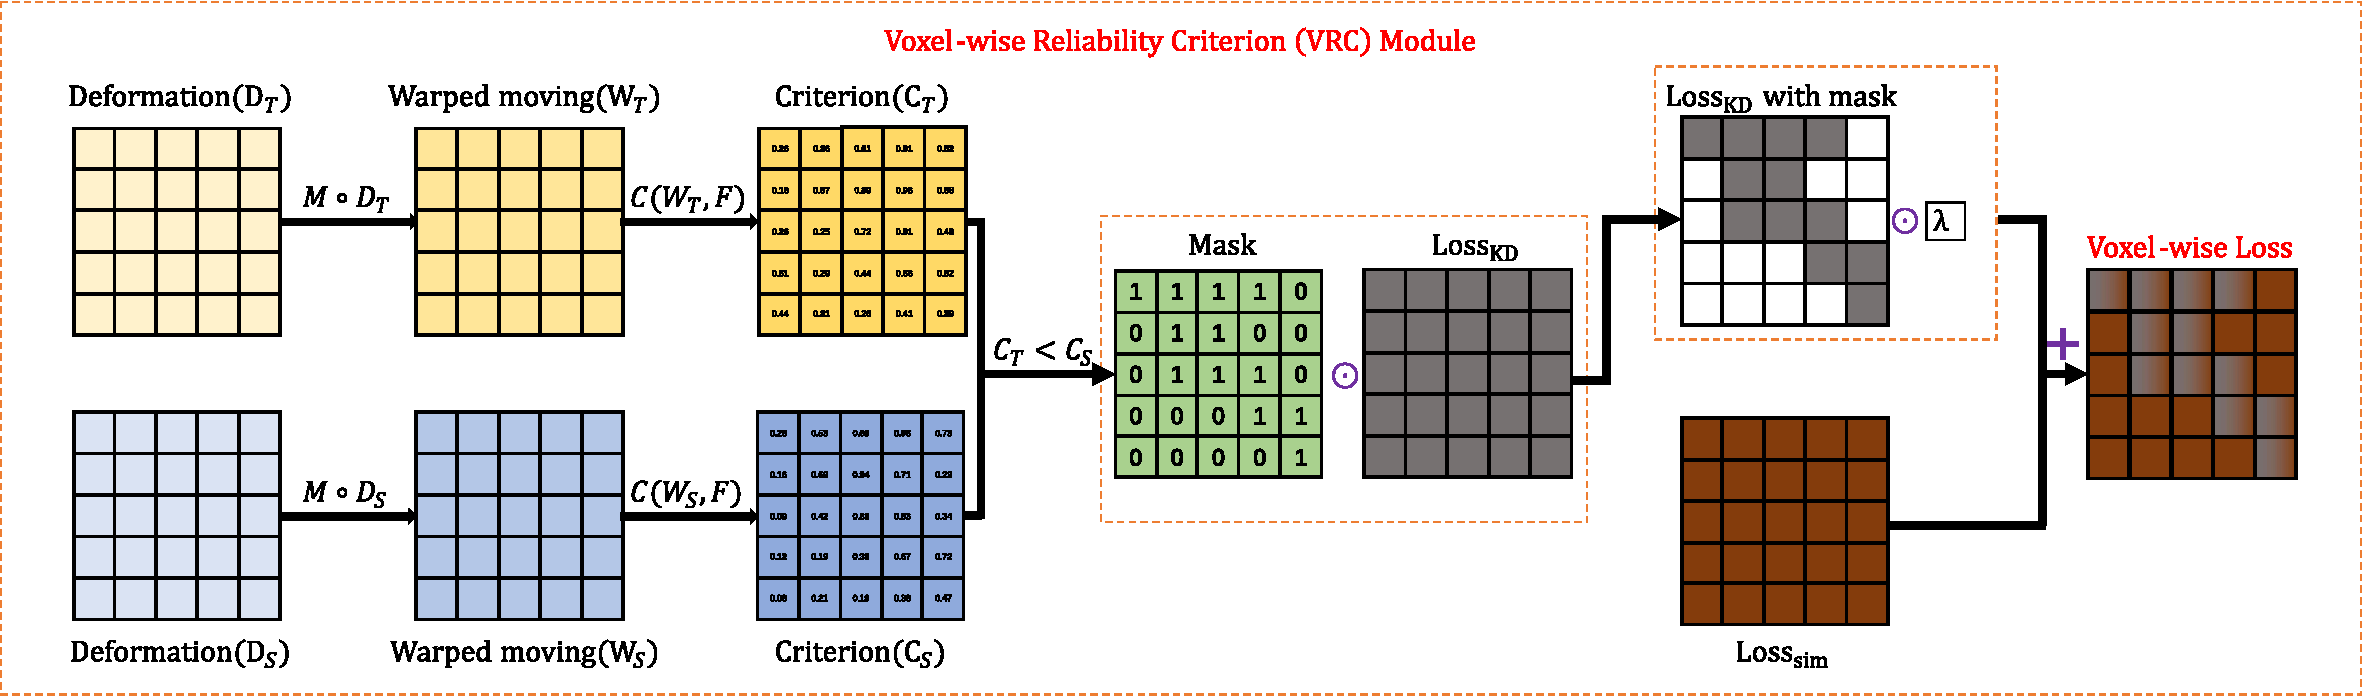
\includegraphics[width=0.9\textwidth]{fig3-vrc-crop.pdf}
    \caption{VRC模块,以图\ref{fig:2}中第二阶段用于微调S的VRC为例}
    \label{fig:3}
\end{figure}

\section{消融实验目的}

在基于金字塔结构的迭代优化医学图像配准方法研究中,MutualReg互学习框架通过教师网络(PAN网络)与学生网络(RegCST网络)的递归式知识蒸馏,实现了无监督配准性能的提升。然而,在互学习过程中,教师网络生成的伪位移场(PFs)可能存在局部区域的误差或不一致性,若直接将其用于监督学生网络的训练,可能导致误差积累或模型性能的退化。因此,VRC(Voxel-wise Reliability Criterion)模块被引入框架中,其核心作用在于筛选出教师网络中可靠性更高的体素位置,仅保留这些位置的位移场信息用于知识蒸馏。具体而言,VRC通过对比教师网络与学生网络生成的形变场对固定图像的匹配程度(基于MIND相似性准则),动态生成掩膜以过滤不可靠的体素,从而优化知识蒸馏的监督信号。

消融实验的核心目的是验证VRC模块在MutualReg框架中的必要性及其对配准性能的实际贡献。由于VRC模块直接影响知识蒸馏过程中监督信号的可靠性,若其有效性未得到充分验证,则无法确定互学习框架的性能提升是源于网络结构的优化还是VRC的引入。此外,通过对比有无VRC模块的实验结果,可以进一步揭示互学习过程中局部误差传递的潜在风险,以及VRC模块在抑制此类风险中的作用机制。例如,若未使用VRC模块,学生网络可能受到教师网络中低质量位移场的误导,导致配准精度下降或形变场平滑性受损。因此,本实验旨在通过定量与定性分析,明确VRC模块在提升配准精度、优化形变场质量方面的具体效果,并为框架的优化提供实证依据。

\section{消融实验设计}

为系统评估VRC模块的有效性,本研究设计了对比实验,重点分析VRC模块对互学习过程的影响。实验采用控制变量法,保持网络结构、训练数据及超参数设置一致,仅改变知识蒸馏损失的监督方式。具体而言,设计以下两种实验条件:

\begin{enumerate}
    \item 无VRC模块的基础互学习:仅使用MIND相似性损失与未加掩膜的知识蒸馏损失(KD损失)进行训练,即直接通过均方误差(MSE)对齐教师网络与学生网络的位移场
    \item 引入VRC模块的优化互学习:在KD损失中引入VRC模块生成的体素掩膜,仅保留教师网络中可靠性高于学生网络的体素位置进行监督
\end{enumerate}

两种实验均基于经过预处理后的LUMIR数据集进行训练。并在LPBA40数据集上进行测试,该数据集包含40例脑部MRI图像,并提供了精细的解剖结构标注,适用于评估多器官配准的准确性。

在训练流程上,教师网络(PAN)与学生网络(RegCST)首先分别进行无监督预训练,随后进入互学习阶段。两种实验条件下,互学习的递归训练轮次均设置为一轮,以确保对比的公平性。模型性能通过两项指标进行量化评估:

\begin{enumerate}
    \item \textbf{配准精度}:采用Dice相似系数衡量配准后解剖结构的对齐程度,计算所有标注器官的平均值
    \item \textbf{形变场平滑性}:通过位移场对数雅可比行列式的标准差(SDlogJ)评估形变场的局部畸变程度,数值越低表明形变越平滑合理
\end{enumerate}

通过上述设计,实验能够从定量指标与定性分析两个层面,全面揭示VRC模块在抑制噪声监督、提升知识蒸馏效率方面的关键作用,进而为MutualReg框架的优化提供理论支持与实践指导。

\section{实验过程与结果分析}

实验在LUMIR脑部MRI数据集上展开,旨在验证VRC模块对互学习框架性能的影响。训练过程中,教师网络(PAN)与学生网络(RegCST)首先分别进行无监督预训练,采用MIND相似性损失与扩散正则化损失联合优化形变场。预训练完成后,进入互学习阶段,两个网络通过递归训练交替优化。为控制变量,实验设置保持一致的训练轮次、学习率衰减策略及批量大小,仅通过是否启用VRC模块区分实验组与对照组。

在无VRC模块的对照组中,学生网络的训练损失由MIND相似性损失与未加掩膜的知识蒸馏损失(KD损失)直接叠加构成。此时,教师网络生成的位移场全部用于监督学生网络,可能导致局部误差传递。实验结果显示,经过一轮互学习后,RegCST网络在验证集上的平均Dice系数为70.9\%,表明其能够有效对齐脑部解剖结构,但仍有提升空间。形变场平滑性指标SDlogJ为0.139,反映出位移场的局部畸变处于合理范围内。

相比之下,启用VRC模块的实验组在知识蒸馏过程中引入了动态掩膜机制。掩膜覆盖区域主要集中解剖结构边缘等特征显著的位置,表明VRC模块倾向于保留教师网络在结构清晰区域的可靠监督信号,同时屏蔽模糊或低对比度区域的噪声干扰。经过一轮互学习后,RegCST网络的Dice系数提升至71.7\%,较对照组提高0.8个百分点,且解剖结构的对齐一致性在视觉评估中表现更优。同时,SDlogJ指标略微上升至0.145,暗示形变场的局部平滑性略有下降。这一现象可能源于VRC模块选择性强化了特定区域的监督,导致位移场在掩膜覆盖区域的梯度变化更为剧烈。尽管如此,SDlogJ的增幅较小(约4.3\%),且未超出临床可接受范围,表明VRC模块在精度与平滑性之间实现了有效权衡。


\section{本章小结}

本章详细分析了医学图像配准方法中的VRC模块及其在MutualReg互学习框架中的作用与效果。首先,介绍了VRC模块的设计思路和工作流程。VRC模块的核心目的是在教师网络生成的位移场对学生网络进行监督时,通过动态筛选体素位置,保留可靠位置的位移场信息,从而提高相互学习的效率。之后,阐述了进行消融实验的目的所在,以及其必要性。消融实验旨在验证VRC模块对MutualReg框架性能的实际贡献。若VRC模块能有效提升配准精度且可降低不可靠监督的风险,则可证明其在互学习框架中的重要性。通过设定有无VRC模块的对比实验,消融实验为分析局部误差传递风险的抑制以及知识蒸馏效率的优化提供了直接证据。然后,实验设计部分描述了控制变量法的实施细节,实验在LPBA40数据集上进行,仅改变损失的监督方式。对照组中不使用VRC模块;而实验组则通过VRC掩膜机制。经过测试,实验结果表明,引入VRC模块后,配准精度有显著提升,从而增强了解剖结构的对齐一致性。同时,对形变场平滑性的影响保持在可接受范围内。掩膜机制的细节探讨进一步揭示了VRC模块在互学习框架中的作用,其倾向在结构清晰的区域保留监督,避免模糊区域误导学生网络。本章通过对VRC模块的分析与实验验证,显示了其在优化知识蒸馏和提升配准精度中的关键作用。

\chapter{互学习优化}

\section{互学习优化实验设计}

互学习优化的核心目标是通过教师网络(PAN)与学生网络(RegCST)的递归式交互训练,实现双向知识蒸馏与性能迭代提升。实验设计围绕两个关键环节展开:首先,构建基于VRC模块的监督损失函数,确保教师网络的高质量位移场能够有效指导学生网络的优化;其次,通过多轮递归训练逐步增强网络的配准能力。在具体实现中,教师网络采用基于金字塔结构与自注意力机制的架构,擅长捕捉多尺度解剖特征,而学生网络基于CNN与迭代优化模块,侧重于局部形变场的精细化预测。两者的互学习过程摒弃了传统自监督策略中依赖自身输出的模式,转而通过跨网络的知识融合实现误差修正与性能互补。

以第二阶段对S网络(这里是RegCST网络)的优化为例,其总损失函数由两部分构成:一是基于MIND相似性度量的无监督损失$\mathcal{L}_{sim}$,用于衡量配准后图像与固定图像的结构对齐程度;二是通过VRC模块加权的知识蒸馏损失$\mathcal{L}_{kd}$,用于对齐指导网络生成的位移场。

具体而言,损失函数可表示为公式\ref{eq:7-2},

\begin{equation}
    \mathcal{L}_{ml}^{RegCST}=\mathcal{L}_{sim}(I_f,I_m\circ \phi_{RegCST})+\lambda\mathcal{L}_{kd}(\phi_{PAN},\phi_{RegCST})\odot Mask
    \label{eq:7-2}
\end{equation}

其中$\lambda$为权重系数,$Mask$为VRC模块生成的体素级掩膜。该掩膜通过对比教师与学生网络的位移场可靠性,动态屏蔽低置信度区域的监督信号,从而避免噪声传递。同理,教师网络在优化过程中亦以相同机制接受学生网络的监督,形成双向知识蒸馏的闭环。两网络通过交替训练与参数更新,逐步收敛至更优的配准状态。





\section{实验过程与结果分析}

为验证互学习优化的有效性,实验在经过预处理后的LUMIR数据集上进行,采用LPBA40脑部MRI数据集进行评测,基准对比模型包括预训练的独立RegCST网络,以及经典配准方法SyN与VoxelMorph。评估指标涵盖定量与定性两个维度:定量方面,采用Dice系数衡量配准精度,SDlogJ评估形变场平滑性;定性方面,通过配准结果的可视化对比分析解剖边界的对齐效果。实验设置中,递归训练轮次逐步增加至三轮,以探究性能随迭代次数的变化趋势。

如表\ref{tab:7-1},首轮训练后RegCST网络的Dice提升至71.7\%,SDlogJ为0.145。随着递归训练轮次增加,互学习优化的累积效应逐步显现。第二轮训练后,RegCST网络的Dice进一步提升至72.3\%,SDlogJ降至0.142;第三轮训练后,Dice达到72.5\%,SDlogJ进一步优化至0.139。这一趋势表明,递归训练不仅通过多轮知识蒸馏细化位移场精度,还借助正则化损失逐步抑制形变场的局部畸变。

\begin{table}[h]
    \centering
    \caption{模型性能定量对比}
    \label{tab:7-1}
    \begin{tabular}{lcc}
        \toprule
        \textbf{模型}         & \textbf{Dice} & \textbf{SDlogJ} \\
        \midrule
        VoxelMorph          & 71.0\%        & 0.134           \\
        SyN                 & 62.8\%        & 0.08            \\
        RegCST(origin)      & 69.8\%        & 0.135           \\
        RegCST(pre-trained) & 70.6\%        & 0.137           \\
        RegCST(R1)          & 71.7\%        & 0.145           \\
        RegCST(R2)          & 72.3\%        & 0.142           \\
        RegCST(R3)          & 72.5\%        & 0.139           \\
        \bottomrule
    \end{tabular}
\end{table}



通过将经过位移场形变后运动图像分割标签叠加在固定图像上,图\ref{fig:7-1}显示了经过三轮递归优化后模型配准结果的可视化展示。尽管固定图像和运动图像之间的变形较大且复杂,但优化后的模型成功地匹配了相应的解剖结构,并生成了准确的配准结果。

\begin{figure}[h]
    \centering
    \begin{minipage}{0.3\textwidth}
        \centering
        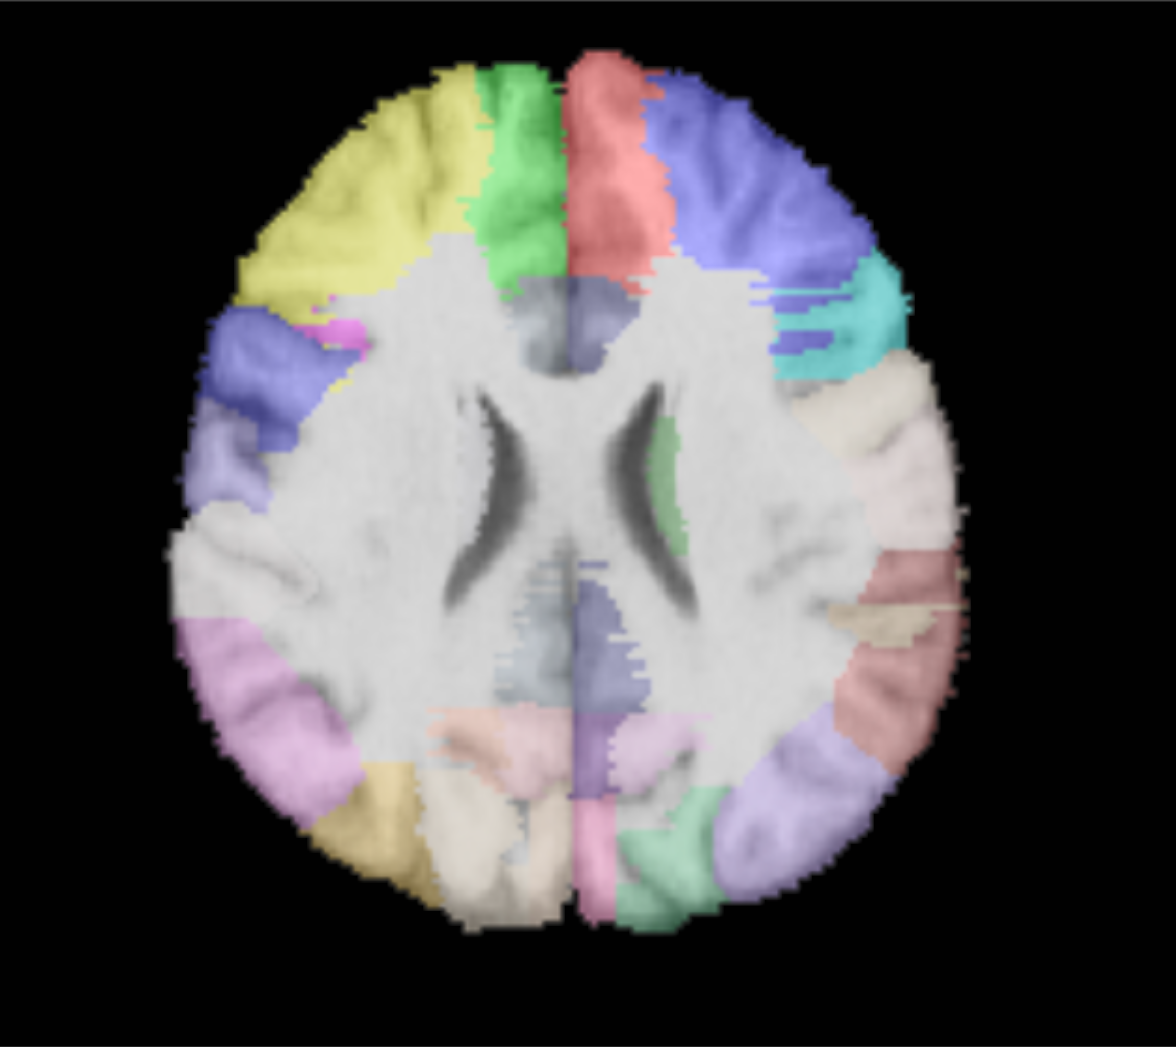
\includegraphics[width=\textwidth]{c7-result1.png}
    \end{minipage}
    \begin{minipage}{0.3\textwidth}
        \centering
        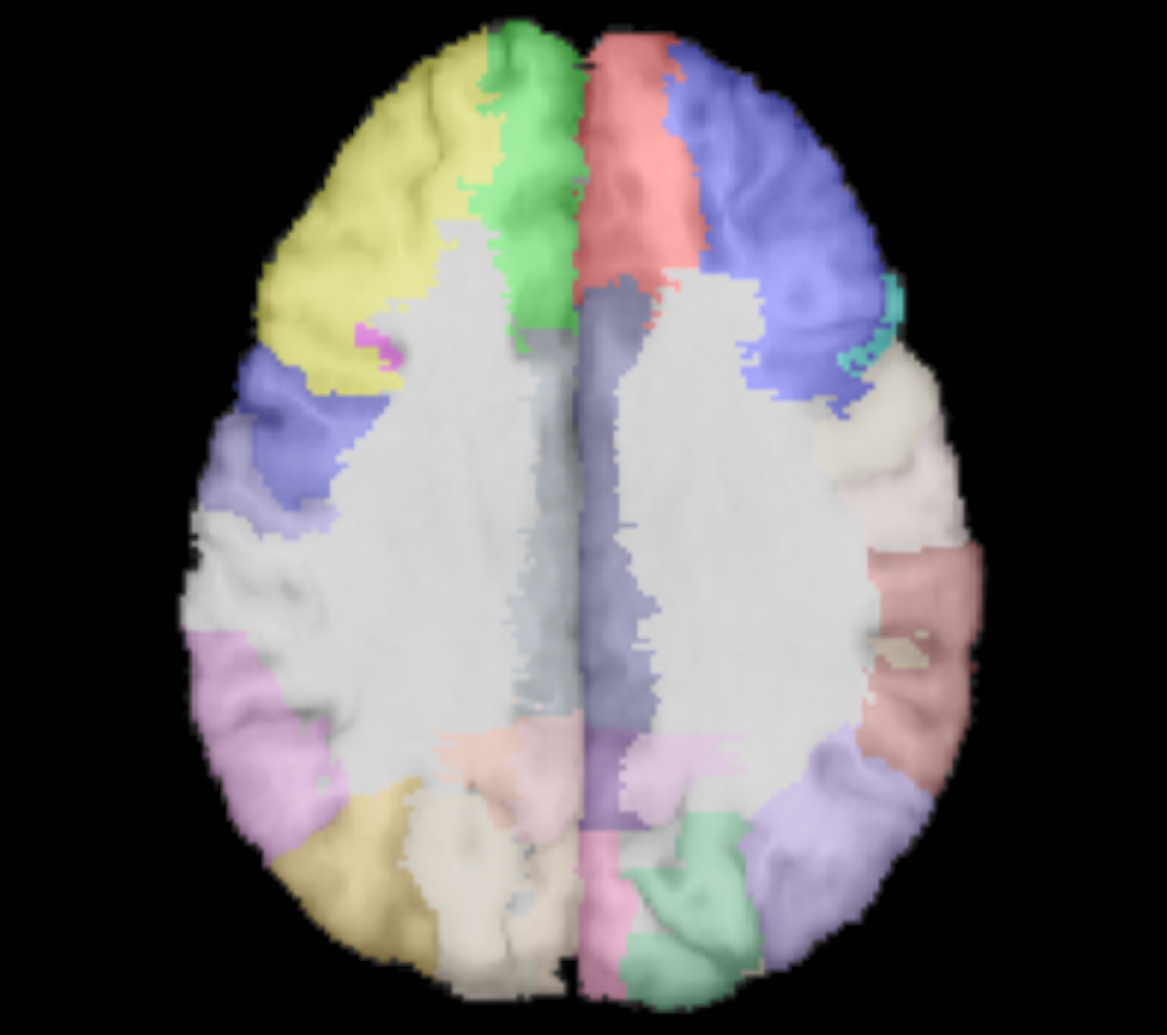
\includegraphics[width=\textwidth]{c7-result2.png}
    \end{minipage}
    \begin{minipage}{0.3\textwidth}
        \centering
        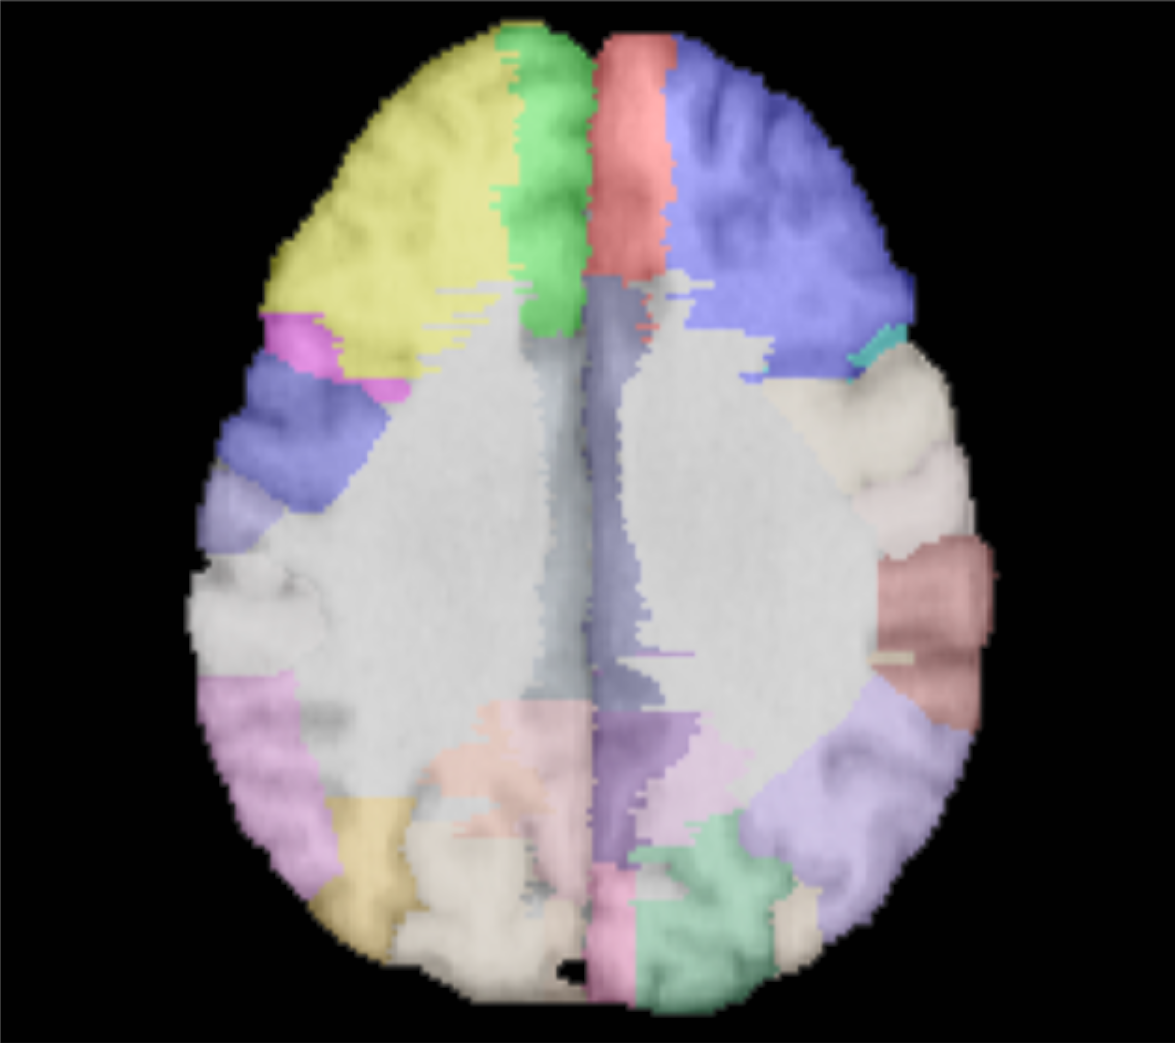
\includegraphics[width=\textwidth]{c7-result3.png}
    \end{minipage}
    \caption{可视化配准结果}
    \label{fig:7-1}
\end{figure}

值得注意的是,SDlogJ的持续下降(三轮降幅达4.1\%)反映出形变场平滑性的系统性改善,可能源于递归训练中扩散正则化的累积效应,或网络对局部梯度冲突的自适应抑制。进一步分析表明,互学习优化的性能增益主要源于两方面:其一,教师网络(PAN)的多尺度特征提取能力为学生网络(RegCST)提供了全局解剖约束,避免其陷入局部最优;其二,VRC模块的动态掩膜机制在递归训练中逐步筛选出更可靠的监督区域。例如,在第二轮训练中,掩膜覆盖率升至32.5\%,且高置信度区域扩展至基底核团等深部结构,推动Dice系数持续上升。此外,双向知识蒸馏促使两网络在迭代中互补优化——PAN网络通过学生网络的反馈增强了局部形变预测的一致性,而RegCST网络则借助教师网络的监督提升了复杂边界的对齐精度。

\section{本章小结}

本章通过设计递归互学习优化框架,研究了教师网络(PAN)与学生网络(RegCST)在双向知识蒸馏中的协同效应。实验结果表明,引入VRC模块的互学习策略能够显著提升配准精度,三轮优化后Dice系数达到72.5\%,较基线模型提升2.3个百分点,且形变场平滑性优于多数传统方法。性能提升的核心机制在于:VRC模块通过动态掩膜抑制低质量监督信号的干扰,而递归训练则通过多轮误差修正与知识融合,逐步增强网络的全局与局部配准能力。然而,实验亦发现递归训练的收益随轮次增加呈现边际递减趋势。例如,第三轮训练的Dice增幅仅为0.2个百分点,可能受限于数据集的规模或网络架构的容量。未来工作可通过引入自适应递归终止机制或融合多模态相似性准则进一步提升优化效率。